\chapter{子群}

\section{定义与例子}

研究任何由一组公理定义的数学对象的结构，一个基本方法是研究该对象中同样满足这些公理的子集。我们从讨论群的子群开始这一计划。揭示结构的第二个基本方法，是研究一个对象的商；商群的概念，粗略地说，是把一个群压缩成一个较小群的方法，将在下一章处理。这两个主题将在全书中反复出现：我们会研究群的子群与商群、环的子环与商环、向量空间的子空间与商空间，等等。

\noindent\textbf{定义.} 设 $G$ 是一个群。若 $G$ 的子集 $H$ 非空，并且对乘积和取逆封闭（即 $x,y\in H$ 蕴含 $x^{-1}\in H$ 且 $xy\in H$），则称 $H$ 是 $G$ 的一个\emph{子群}。若 $H$ 是 $G$ 的子群，记作 $H\leq G$。

$G$ 的子群就是 $G$ 的那些子集，它们关于 $G$ 中定义的运算本身也是群；也就是说，$G$ 上的二元运算限制到 $H$ 后给出 $H$ 上的二元运算，该运算结合，在 $H$ 中有单位元，并且 $H$ 的每个元素在 $H$ 中有逆元。

当我们说 $H$ 是 $G$ 的子群时，总是指 $H$ 上的群运算是 $G$ 上的运算限制到 $H$ 得到的运算（一般说来，子集 $H$ 也可能关于某个不同于 $G$ 的限制运算的运算而具有群结构，参见下面例 5(a)）。正如我们对函数限制到子集时所做的那样，我们用同一个符号表示 $G$ 的运算和子群 $H$ 的运算。若 $H\leq G$ 且 $H\neq G$，则写作 $H<G$，以强调包含是真包含。

若 $H$ 是 $G$ 的子群，则由于 $H$ 的运算是 $G$ 的运算在 $H$ 上的限制，$H$ 中的任何等式也可看作 $G$ 中的等式。因此，$G$ 中的消去律说明：$H$ 的单位元与 $G$ 的单位元相同（特别地，每个子群都必须含有 $1$，即 $G$ 的单位元）；并且 $H$ 中元素 $x$ 的逆元，与把 $x$ 看作 $G$ 中元素时的逆元相同（所以记号 $x^{-1}$ 没有歧义）。

\paragraph{例}
\begin{enumerate}[label=(\arabic*)]
  \item 在加法运算下，$\ZZ\leq \QQ$ 且 $\QQ\leq \RR$。
  \item 任意群 $G$ 都有两个子群：$H=G$ 和 $H=\{1\}$；后者称为\emph{平凡子群}，今后记作 $1$。
  \item 若 $G=D_{2n}$ 是阶为 $2n$ 的二面体群，令 $H=\{1,r,r^2,\ldots,r^{n-1}\}$ 为 $G$ 中所有旋转组成的集合。由于两个旋转的乘积仍是旋转，旋转的逆仍是旋转，所以 $H$ 是 $D_{2n}$ 的一个阶为 $n$ 的子群。
  \item 偶整数集合是所有整数在加法下构成的群的一个子群。
  \item 以下是一些不是子群的子集的例子：
  \begin{enumerate}[label=(\alph*)]
    \item $\QQ-\{0\}$ 在乘法下不是 $\RR$ 在加法下的子群，尽管二者都是群且 $\QQ-\{0\}$ 是 $\RR$ 的子集；$\QQ-\{0\}$ 上的乘法不是 $\RR$ 上加法的限制。
    \item $\ZZ^+$（在加法下）不是 $\ZZ$（在加法下）的子群，因为虽然 $\ZZ^+$ 对 $+$ 封闭，但它不含 $\ZZ$ 的单位元 $0$；并且虽然每个 $x\in\ZZ^+$ 在 $\ZZ$ 中有加法逆元 $-x$，但 $-x\notin\ZZ^+$，即 $\ZZ^+$ 对取逆不封闭（特别地，$\ZZ^+$ 在加法下不是群）。基于类似原因，$(\ZZ-\{0\},\times)$ 不是 $(\QQ-\{0\},\times)$ 的子群。
    \item $D_6$ 不是 $D_8$ 的子群，因为前者甚至不是后者的子集。
  \end{enumerate}
  \item “是……的子群”这一关系具有传递性：若 $H$ 是群 $G$ 的子群，$K$ 是 $H$ 的子群，则 $K$ 也是 $G$ 的子群。
\end{enumerate}

正如我们在第 1 章看到的，即使在简单例子中，检查某个给定二元运算是否满足所有群公理（尤其是结合律）也可能相当繁琐。然而，一旦我们知道已经有一个群，要检查其中某个子集是否为子群就容易得多，因为只需检查它是否对乘法和取逆封闭。下一个命题说明这两个条件可合并为一个检验；并且对于有限群，只需检查乘法封闭即可。

\medskip
\noindent\textbf{命题 1（子群判别法）.} 群 $G$ 的子集 $H$ 是子群，当且仅当
\begin{enumerate}[label=(\arabic*)]
  \item $H\neq\varnothing$；
  \item 对所有 $x,y\in H$，$xy^{-1}\in H$。
\end{enumerate}
此外，若 $H$ 是有限集，则只需检查 $H$ 非空且对乘法封闭。

\begin{proof}
若 $H$ 是 $G$ 的子群，则 (1) 和 (2) 显然成立，因为 $H$ 含有 $G$ 的单位元、含有每个元素的逆元，并且对乘法封闭。

反过来，假设 $H$ 满足 (1) 和 (2)，我们证明 $H\leq G$。取 $H$ 中任意元素 $x$（由 (1) 可取）。令 $y=x$ 并应用 (2)，得 $1=xx^{-1}\in H$，所以 $H$ 含有 $G$ 的单位元。再由 (2)，由于 $H$ 含有 $1$ 和 $x$，$H$ 含有元素 $1x^{-1}$，即 $x^{-1}\in H$，所以 $H$ 对取逆封闭。最后，若 $x,y$ 是 $H$ 的任意两个元素，则由刚才证明，$y^{-1}\in H$；再由 (2)，$H$ 也含有 $x(y^{-1})^{-1}=xy$。因此 $H$ 也对乘法封闭，从而 $H$ 是 $G$ 的子群。

现在假设 $H$ 有限且对乘法封闭，取任意 $x\in H$。在 $x,x^2,x^3,\ldots$ 中只有有限多个不同元素，所以存在整数 $a,b$，$b>a$，使得 $x^a=x^b$。若 $n=b-a$，则 $x^n=1$，因此 $H$ 中每个元素都有有限阶。于是 $x^{n-1}=x^{-1}$ 属于 $H$，所以 $H$ 自动对取逆封闭。
\end{proof}

\subsection*{练习}

设 $G$ 是一个群。
\begin{enumerate}[label=\arabic*.]
  \item 在 (a)--(e) 中，证明指定子集是给定群的子群：
  \begin{enumerate}[label=(\alph*)]
    \item 形如 $a+ai$、$a\in\RR$ 的复数集合（在加法下）；
    \item 绝对值为 $1$ 的复数集合，即复平面中的单位圆（在乘法下）；
    \item 对固定 $n\in\ZZ^+$，所有分母整除 $n$ 的有理数集合（在加法下）；
    \item 对固定 $n\in\ZZ^+$，所有分母与 $n$ 互素的有理数集合（在加法下）；
    \item 所有平方为有理数的非零实数集合（在乘法下）。
  \end{enumerate}
  \item 在 (a)--(e) 中，证明指定子集不是给定群的子群：
  \begin{enumerate}[label=(\alph*)]
    \item 当 $n\geq 3$ 时，$S_n$ 中所有 $2$-轮换的集合；
    \item 当 $n\geq 3$ 时，$D_{2n}$ 中所有反射的集合；
    \item 对复合整数 $n>1$ 和一个含有阶为 $n$ 的元素的群 $G$，集合
    \[
      \{x\in G\mid |x|=n\}\cup\{1\};
    \]
    \item $\ZZ$ 中所有正、负奇整数与 $0$ 合在一起的集合；
    \item 平方为有理数的实数集合（在加法下）。
  \end{enumerate}
  \item 证明二面体群 $D_8$ 的下列子集实际上是子群：
  \[
    \text{(a) }\{1,r^2,s,sr^2\},\qquad
    \text{(b) }\{1,r^2,sr,sr^3\}.
  \]
  \item 给出一个群 $G$ 和一个无限子集 $H$ 的具体例子，使得 $H$ 对群运算封闭，但不是 $G$ 的子群。
  \item 证明若 $n=|G|>2$，则 $G$ 不可能有一个满足 $|H|=n-1$ 的子群 $H$。
  \item 设 $G$ 是阿贝尔群。证明
  \[
    \{g\in G\mid |g|<\infty\}
  \]
  是 $G$ 的子群（称为 $G$ 的\emph{挠子群}）。给出一个具体例子说明，当 $G$ 非阿贝尔时，这个集合不一定是子群。
  \item 固定整数 $n>1$。求 $\ZZ\times(\ZZ/n\ZZ)$ 的挠子群（参见上一题）。说明无限阶元素再加上单位元组成的集合不是这个直积的子群。
  \item 设 $H$ 和 $K$ 是 $G$ 的子群。证明 $H\cup K$ 是子群，当且仅当 $H\subseteq K$ 或 $K\subseteq H$。
  \item 设 $G=\GL_n(F)$，其中 $F$ 是任意域。定义
  \[
    \SL_n(F)=\{A\in \GL_n(F)\mid \det(A)=1\}
  \]
  （称为\emph{特殊线性群}）。证明 $\SL_n(F)\leq \GL_n(F)$。
  \item \begin{enumerate}[label=(\alph*)]
    \item 证明若 $H$ 与 $K$ 是 $G$ 的子群，则交 $H\cap K$ 也是 $G$ 的子群。
    \item 证明 $G$ 的任意非空子群族的交仍是 $G$ 的子群（不要假设该族可数）。
  \end{enumerate}
  \item 设 $A$ 和 $B$ 是群。证明下列集合是直积 $A\times B$ 的子群：
  \begin{enumerate}[label=(\alph*)]
    \item $\{(a,1)\mid a\in A\}$；
    \item $\{(1,b)\mid b\in B\}$；
    \item $\{(a,a)\mid a\in A\}$，这里假设 $B=A$（称为\emph{对角子群}）。
  \end{enumerate}
  \item 设 $A$ 是阿贝尔群，固定 $n\in\ZZ$。证明下列集合是 $A$ 的子群：
  \[
    \text{(a) }\{a^n\mid a\in A\},\qquad
    \text{(b) }\{a\in A\mid a^n=1\}.
  \]
  \item 设 $H$ 是有理数加法群的一个子群，并满足对 $H$ 的每个非零元素 $x$ 都有 $1/x\in H$。证明 $H=0$ 或 $H=\QQ$。
  \item 证明 $\{x\in D_{2n}\mid x^2=1\}$ 不是 $D_{2n}$ 的子群（这里 $n\geq 3$）。
  \item 设 $H_1\leq H_2\leq\cdots$ 是 $G$ 的一个升链子群。证明 $\bigcup_{i=1}^{\infty}H_i$ 是 $G$ 的子群。
  \item 设 $n\in\ZZ^+$，$F$ 是一个域。证明集合
  \[
    \{(a_{ij})\in\GL_n(F)\\mid a_{ij}=0\text{ 对所有 }i>j\}
  \]
  是 $\GL_n(F)$ 的一个子群（称为\emph{上三角矩阵群}）。
  \item 设 $n\in\ZZ^+$，$F$ 是一个域。证明集合
  \[
    \{(a_{ij})\in\GL_n(F)\mid a_{ij}=0\text{ 对所有 }i>j,\text{ 且 }a_{ii}=1\text{ 对所有 }i\}
  \]
  是 $\GL_n(F)$ 的一个子群。
\end{enumerate}

\section{中心化子与正规化子，稳定子与核}

现在我们引入任意群 $G$ 中一些重要的子群族；它们尤其提供许多子群的例子。设 $A$ 是 $G$ 的任意非空子集。

\noindent\textbf{定义.} 定义
\[
  C_G(A)=\{g\in G\mid gag^{-1}=a\text{ 对所有 }a\in A\}.
\]
这个 $G$ 的子集称为 $A$ 在 $G$ 中的\emph{中心化子}。由于 $gag^{-1}=a$ 当且仅当 $ga=ag$，$C_G(A)$ 就是 $G$ 中与 $A$ 的每个元素都交换的那些元素组成的集合。

我们证明 $C_G(A)$ 是 $G$ 的子群。首先，$C_G(A)\neq\varnothing$，因为 $1\in C_G(A)$：单位元的定义给出 $1a=a1$ 对所有 $a\in G$ 成立，特别地对所有 $a\in A$ 成立，所以 $1$ 满足属于 $C_G(A)$ 的定义条件。其次，假设 $x,y\in C_G(A)$，即对所有 $a\in A$，有 $xax^{-1}=a$ 且 $yay^{-1}=a$（注意，这并不意味着 $xy=yx$）。先观察到，由 $yay^{-1}=a$，先左乘 $y^{-1}$ 再右乘 $y$ 并化简，得到 $a=y^{-1}ay$；也就是说，$y^{-1}\in C_G(A)$，所以 $C_G(A)$ 对取逆封闭。现在
\begin{align*}
  (xy)a(xy)^{-1}
  &= (xy)a(y^{-1}x^{-1}) &&\text{（由命题 1.1(4) 用于 $(xy)^{-1}$）}\\
  &= x(yay^{-1})x^{-1} &&\text{（结合律）}\\
  &= xax^{-1} &&\text{（因为 $y\in C_G(A)$）}\\
  &= a &&\text{（因为 $x\in C_G(A)$），}
\end{align*}
所以 $xy\in C_G(A)$，$C_G(A)$ 对乘积封闭，故 $C_G(A)\leq G$。

在特殊情形 $A=\{a\}$ 下，我们简写 $C_G(a)$ 而不是 $C_G(\{a\})$。此时对所有 $n\in\ZZ$，都有 $a^n\in C_G(a)$。

例如，在阿贝尔群 $G$ 中，对所有子集 $A$，有 $C_G(A)=G$。通过检查可得 $C_{Q_8}(i)=\{\pm1,\pm i\}$。练习中还会给出若干其他例子。

稍后我们会讨论如何减少计算中心化子（以及其他类似性质的子群）时看起来必不可少的单个群元素之间交换性的检查。

\noindent\textbf{定义.} 定义
\[
  Z(G)=\{g\in G\mid gx=xg\text{ 对所有 }x\in G\},
\]
即与 $G$ 中所有元素都交换的元素集合。这个 $G$ 的子集称为 $G$ 的\emph{中心}。注意 $Z(G)=C_G(G)$，所以上面的论证把 $Z(G)\leq G$ 作为特殊情形证明了。读者也可直接证明 $Z(G)$ 是子群。

\noindent\textbf{定义.} 定义
\[
  gAg^{-1}=\{gag^{-1}\mid a\in A\}.
\]
定义 $A$ 在 $G$ 中的\emph{正规化子}为
\[
  N_G(A)=\{g\in G\mid gAg^{-1}=A\}.
\]

注意若 $g\in C_G(A)$，则对所有 $a\in A$ 有 $gag^{-1}=a\in A$，所以 $C_G(A)\leq N_G(A)$。证明 $N_G(A)$ 是 $G$ 的子群，与证明 $C_G(A)\leq G$ 的步骤相同，只需作适当修改。

\paragraph{例}
\begin{enumerate}[label=(\arabic*)]
  \item 若 $G$ 是阿贝尔群，则 $G$ 中所有元素都交换，所以 $Z(G)=G$。类似地，对 $G$ 的任意子集 $A$，$C_G(A)=N_G(A)=G$，因为对每个 $g\in G$ 和每个 $a\in A$，都有 $gag^{-1}=gg^{-1}a=a$。
  \item 设 $G=D_8$ 是阶为 $8$ 的二面体群，有通常的生成元 $r$ 和 $s$；设 $A=\{1,r,r^2,r^3\}$ 为 $D_8$ 中旋转构成的子群。我们说明 $C_{D_8}(A)=A$。由于 $r$ 的各个幂彼此交换，$A\leq C_{D_8}(A)$。由于 $sr=r^{-1}s\neq rs$，元素 $s$ 不与 $A$ 的所有成员交换，即 $s\notin C_{D_8}(A)$。最后，$D_8$ 中不属于 $A$ 的元素都形如 $sr^i$，其中 $i\in\{0,1,2,3\}$。若元素 $sr^i$ 属于 $C_{D_8}(A)$，则由于 $C_{D_8}(A)$ 是含有 $r$ 的子群，也会有
  \[
    s=(sr^i)(r^{-i})\in C_{D_8}(A),
  \]
  这与上面矛盾。因此 $C_{D_8}(A)=A$。
  \item 仍如前例，令 $G=D_8$ 且 $A=\{1,r,r^2,r^3\}$。我们说明 $N_{D_8}(A)=D_8$。一般地，子集的中心化子包含于其正规化子，所以 $A\leq N_{D_8}(A)$。再计算
  \[
    sAs^{-1}=\{s1s^{-1},srs^{-1},sr^2s^{-1},sr^3s^{-1}\}
    =\{1,r^3,r^2,r\}=A,
  \]
  因此 $s\in N_{D_8}(A)$。（注意，集合 $sAs^{-1}$ 等于集合 $A$，尽管两个集合中的元素出现顺序不同；这是因为 $s$ 在 $A$ 的正规化子中，但不在 $A$ 的中心化子中。）现在 $r$ 和 $s$ 都属于子群 $N_{D_8}(A)$，所以对所有整数 $i,j$，$s^jr^i\in N_{D_8}(A)$；也就是说，$D_8$ 的每个元素都在 $N_{D_8}(A)$ 中（回忆 $r$ 和 $s$ 生成 $D_8$）。既然 $D_8\leq N_{D_8}(A)$，而反向包含由正规化子定义显然成立，故 $N_{D_8}(A)=D_8$。
  \item 我们说明 $D_8$ 的中心是子群 $\{1,r^2\}$。首先，任意群 $G$ 的中心都包含于 $C_G(A)$，其中 $A$ 是 $G$ 的任意子集。于是由例 2，
  \[
    Z(D_8)\leq C_{D_8}(A)=A,
  \]
  其中 $A=\{1,r,r^2,r^3\}$。例 2 中的计算说明 $r$，同样 $r^3$，不在 $Z(D_8)$ 中，所以 $Z(D_8)\leq\{1,r^2\}$。为证明反向包含，注意 $r$ 与 $r^2$ 交换，并且直接计算可得 $s$ 也与 $r^2$ 交换。由于 $r$ 与 $s$ 生成 $D_8$，$D_8$ 中每个元素都与 $r^2$（以及 $1$）交换，因此 $\{1,r^2\}\leq Z(D_8)$，故等号成立。
  \item 设 $G=S_3$，令 $A=\{1,(1\ 2)\}$。我们解释为什么 $C_{S_3}(A)=N_{S_3}(A)=A$。可以直接计算 $C_{S_3}(A)=A$，并用例 2 中的思想减少计算。另一种方法是：由于一个元素与其幂交换，$A\leq C_{S_3}(A)$。由拉格朗日定理（第 1.7 节练习 19），子群 $C_{S_3}(A)$ 的阶整除 $|S_3|=6$。同样把拉格朗日定理应用于 $C_{S_3}(A)$ 的子群 $A$，得 $2$ 整除 $|C_{S_3}(A)|$。唯一的可能是 $|C_{S_3}(A)|=2$ 或 $6$。若为后者，则 $C_{S_3}(A)=S_3$，即 $A\leq Z(S_3)$；这与 $(1\ 2)$ 不与 $(1\ 2\ 3)$ 交换矛盾。因此 $|C_{S_3}(A)|=2$，故 $A=C_{S_3}(A)$。

  接着注意 $N_{S_3}(A)=A$，因为 $\sigma\in N_{S_3}(A)$ 当且仅当
  \[
    \{\sigma1\sigma^{-1},\sigma(1\ 2)\sigma^{-1}\}=\{1,(1\ 2)\}.
  \]
  由于 $\sigma1\sigma^{-1}=1$，这个集合等式成立当且仅当 $\sigma(1\ 2)\sigma^{-1}=(1\ 2)$，也就是当且仅当 $\sigma\in C_{S_3}(A)$。

  $S_3$ 的中心是单位子群，因为 $Z(S_3)\leq C_{S_3}(A)=A$，而 $(1\ 2)\notin Z(S_3)$。
\end{enumerate}

\subsection*{群作用的稳定子与核}

$A$ 在 $G$ 中的正规化子、中心化子以及 $G$ 的中心都是子群这一事实，可作为群作用相关结果的特殊情形推出。这说明 $G$ 的结构会反映在它所作用的集合上。具体地说，若群 $G$ 作用在集合 $S$ 上，且 $s$ 是 $S$ 中的某个固定元素，则 $s$ 在 $G$ 中的\emph{稳定子}是集合
\[
  G_s=\{g\in G\mid g\cdot s=s\}
\]
（参见第 1.7 节练习 4）。我们简要说明 $G_s\leq G$：首先，由作用公理 (2)，$1\in G_s$。此外，若 $y\in G_s$，则
\begin{align*}
  s &= 1\cdot s=(y^{-1}y)\cdot s\\
    &= y^{-1}\cdot (y\cdot s) &&\text{（由作用公理 (1)）}\\
    &= y^{-1}\cdot s &&\text{（因为 $y\in G_s$），}
\end{align*}
所以 $y^{-1}\in G_s$。最后，若 $x,y\in G_s$，则
\begin{align*}
  (xy)\cdot s &= x\cdot(y\cdot s) &&\text{（由作用公理 (1)）}\\
  &=x\cdot s &&\text{（因为 $y\in G_s$）}\\
  &=s &&\text{（因为 $x\in G_s$）。}
\end{align*}
这证明了 $G_s$ 是 $G$ 的子群。类似但更简单的论证证明作用的核也是子群，其中 $G$ 在 $S$ 上作用的\emph{核}定义为
\[
  \{g\in G\mid g\cdot s=s\text{ 对所有 }s\in S\}
\]
（参见第 1.7 节练习 1）。

\paragraph{例}
\begin{enumerate}[label=(\arabic*)]
  \item 群 $G=D_8$ 作用在正方形四个顶点的集合 $A$ 上（参见第 1.7 节例 4）。任意顶点 $a$ 的稳定子是 $D_8$ 的子群 $\{1,t\}$，其中 $t$ 是关于经过顶点 $a$ 与正方形中心的对称轴的反射。这个作用的核是单位子群，因为只有恒等对称固定每个顶点。
  \item 群 $G=D_8$ 也作用在集合 $A$ 上，$A$ 的元素是两对相对顶点的无序对（按第 1.2 节图 2 的标号，$A=\{\{1,3\},\{2,4\}\}$）。$D_8$ 在这个集合 $A$ 上作用的核是子群 $\{1,s,r^2,sr^2\}$；对 $A$ 的任一元素 $a$，$a$ 在 $D_8$ 中的稳定子等于该作用的核。
\end{enumerate}

最后我们观察，中心化子、正规化子以及核是子群这一事实，都是作用的稳定子和核是子群这一事实的特殊情形（这会在第 4 章进一步讨论）。令 $S=\mcP(G)$ 为 $G$ 的所有子集的集合，并令 $G$ 在 $S$ 上按共轭作用：对每个 $g\in G$ 和每个 $B\subseteq G$，令
\[
  g:B\mapsto gBg^{-1},\qquad gBg^{-1}=\{gbg^{-1}\mid b\in B\}
\]
（见第 1.7 节练习 16）。在这个作用下，容易验证 $N_G(A)$ 正是 $A$ 在 $G$ 中的稳定子（即 $N_G(A)=G_s$，其中 $s=A\in\mcP(G)$），所以 $N_G(A)$ 是 $G$ 的子群。

再令群 $N_G(A)$ 在集合 $S=A$ 上按共轭作用，即对所有 $g\in N_G(A)$ 和 $a\in A$，
\[
  g:a\mapsto gag^{-1}.
\]
注意由 $N_G(A)$ 的定义，这确实把 $A$ 映到 $A$，从而给出 $A$ 上的作用。此时容易验证 $C_G(A)$ 正是这个作用的核，因此 $C_G(A)\leq N_G(A)$；由关系“$\leq$”的传递性，$C_G(A)\leq G$。最后，$Z(G)$ 是 $G$ 在 $S=G$ 上按共轭作用的核，所以 $Z(G)\leq G$。

\subsection*{练习}

\begin{enumerate}[label=\arabic*.]
  \item 证明
  \[
    C_G(A)=\{g\in G\mid g^{-1}ag=a\text{ 对所有 }a\in A\}.
  \]
  \item 证明 $C_G(Z(G))=G$，并推出 $N_G(Z(G))=G$。
  \item 证明若 $A$ 与 $B$ 是 $G$ 的子集且 $A\subseteq B$，则 $C_G(B)$ 是 $C_G(A)$ 的子群。
  \item 对 $S_3$、$D_8$ 和 $Q_8$，计算每个元素的中心化子，并求每个群的中心。拉格朗日定理（第 1.7 节练习 19）是否能简化你的工作？
  \item 在 (a)--(c) 中，对指定的群 $G$ 及 $G$ 的子群 $A$，证明 $C_G(A)=A$ 且 $N_G(A)=G$。
  \begin{enumerate}[label=(\alph*)]
    \item $G=S_3$，$A=\{1,(1\ 2\ 3),(1\ 3\ 2)\}$；
    \item $G=D_8$，$A=\{1,s,r^2,sr^2\}$；
    \item $G=D_{10}$，$A=\{1,r,r^2,r^3,r^4\}$。
  \end{enumerate}
  \item 设 $H$ 是群 $G$ 的子群。
  \begin{enumerate}[label=(\alph*)]
    \item 证明 $H\leq N_G(H)$。给出一个例子说明，若 $H$ 不是子群，则该结论不一定成立。
    \item 证明 $H\leq C_G(H)$ 当且仅当 $H$ 是阿贝尔群。
  \end{enumerate}
  \item 设 $n\in\ZZ$ 且 $n\geq 3$。证明：
  \begin{enumerate}[label=(\alph*)]
    \item 若 $n$ 为奇数，则 $Z(D_{2n})=1$；
    \item 若 $n=2k$，则 $Z(D_{2n})=\{1,r^k\}$。
  \end{enumerate}
  \item 令 $G=S_n$，固定 $i\in\{1,2,\ldots,n\}$，并令
  \[
    G_i=\{\sigma\in G\mid \sigma(i)=i\}
  \]
  （即 $i$ 在 $G$ 中的稳定子）。用群作用证明 $G_i$ 是 $G$ 的子群，并求 $|G_i|$。
  \item 对 $G$ 的任意子群 $H$ 和任意非空子集 $A$，定义
  \[
    N_H(A)=\{h\in H\mid hAh^{-1}=A\}.
  \]
  证明 $N_H(A)=N_G(A)\cap H$，并推出 $N_H(A)$ 是 $H$ 的子群（注意 $A$ 不必是 $H$ 的子集）。
  \item 设 $H$ 是 $G$ 中阶为 $2$ 的子群。证明 $N_G(H)=C_G(H)$。推出若 $N_G(H)=G$，则 $H\leq Z(G)$。
  \item 证明对 $G$ 的任意子集 $A$，都有 $Z(G)\leq N_G(A)$。
  \item 设 $R$ 是所有以独立变量 $x_1,x_2,x_3,x_4$ 为变量、整数为系数的多项式集合；也就是说，$R$ 的元素是形如 $a x_1^{r_1}x_2^{r_2}x_3^{r_3}x_4^{r_4}$ 的项的有限和，其中 $a$ 是整数，$r_1,\ldots,r_4$ 是非负整数。例如
  \[
    12x_1^5x_2^7x_4-18x_2^3x_3+11x_1^6x_2^3x_3^2x_4^3 \tag{*}
  \]
  是 $R$ 的一个典型元素。每个 $\sigma\in S_4$ 通过定义 $\sigma\cdot x_i=x_{\sigma(i)}$ 给出 $\{x_1,\ldots,x_4\}$ 的一个置换。将其扩展为从 $R$ 到 $R$ 的映射：
  \[
    \sigma\cdot p(x_1,x_2,x_3,x_4)=p(x_{\sigma(1)},x_{\sigma(2)},x_{\sigma(3)},x_{\sigma(4)})
  \]
  对所有 $p(x_1,x_2,x_3,x_4)\in R$ 成立（即 $\sigma$ 只是置换变量下标）。例如，若 $\sigma=(1\ 2)(3\ 4)$，且 $p$ 是 (*) 中的多项式，则
  \[
    \sigma\cdot p=12x_2^5x_1^7x_3-18x_1^3x_4+11x_2^6x_1^3x_4^2x_3^3
    =12x_1^7x_2^5x_3-18x_1^3x_4+11x_1^3x_2^6x_3^3x_4^2.
  \]
  \begin{enumerate}[label=(\alph*)]
    \item 令 $p=p(x_1,\ldots,x_4)$ 为 (*) 中的多项式，令 $\sigma=(1\ 2\ 3\ 4)$，$\tau=(1\ 2\ 3)$。计算 $\sigma\cdot p$、$\tau\cdot(\sigma\cdot p)$、$(\tau\circ\sigma)\cdot p$ 和 $(\sigma\circ\tau)\cdot p$。
    \item 证明上述定义给出 $S_4$ 在 $R$ 上的一个（左）群作用。
    \item 列出 $S_4$ 中所有稳定 $x_4$ 的置换，并证明它们构成一个同构于 $S_3$ 的子群。
    \item 列出 $S_4$ 中所有稳定 $x_1+x_2$ 的置换，并证明它们构成一个阶为 $4$ 的阿贝尔子群。
    \item 列出 $S_4$ 中所有稳定 $x_1x_2+x_3x_4$ 的置换，并证明它们构成一个同构于阶为 $8$ 的二面体群的子群。
    \item 说明稳定 $(x_1+x_2)(x_3+x_4)$ 的 $S_4$ 中的置换，恰好与 (e) 中得到的置换相同。（(e) 和 (f) 中出现的两个多项式及稳定它们的子群，将在第 14.6 节研究四次方程的根时起重要作用。）
  \end{enumerate}
  \item 设 $n$ 是正整数，$R$ 是所有以独立变量 $x_1,x_2,
  \ldots,x_n$ 为变量、整数为系数的多项式集合。对每个 $\sigma\in S_n$ 定义映射
  \[
    \sigma:R\to R,
    \qquad
    \sigma\cdot p(x_1,x_2,\ldots,x_n)=p(x_{\sigma(1)},x_{\sigma(2)},\ldots,x_{\sigma(n)}).
  \]
  证明这定义了 $S_n$ 在 $R$ 上的一个（左）群作用。
  \item 设 $H(F)$ 为第 1.4 节练习 11 中引入的域 $F$ 上的海森堡群。确定哪些矩阵属于 $H(F)$ 的中心，并证明 $Z(H(F))$ 同构于 $F$ 的加法群。
\end{enumerate}

\section{循环群与循环子群}

设 $G$ 是任意群，$x$ 是 $G$ 的任意元素。构造 $G$ 的子群 $H$ 的一种方式，是令 $H$ 为 $x$ 的所有整数次幂（正次幂、负次幂和零次幂）组成的集合；至少就 $x$ 而言，这保证了对取逆和乘积封闭。本节研究由一个元素生成的群。

\noindent\textbf{定义.} 群 $H$ 称为\emph{循环的}，如果 $H$ 可由单个元素生成；也就是说，存在某个 $x\in H$，使得
\[
  H=\{x^n\mid n\in\ZZ\}
\]
（像往常一样，这里运算写成乘法）。

若用加法记号，则 $H$ 循环表示 $H=\{nx\mid n\in\ZZ\}$。两种情形中我们都写 $H=\langle x\rangle$，并称 $H$ 由 $x$ 生成（$x$ 是 $H$ 的生成元）。一个循环群可以有不止一个生成元。例如，若 $H=\langle x\rangle$，则也有 $H=\langle x^{-1}\rangle$，因为 $(x^{-1})^n=x^{-n}$，而当 $n$ 遍历所有整数时，$-n$ 也遍历所有整数，所以
\[
  \{x^n\mid n\in\ZZ\}=\{(x^{-1})^n\mid n\in\ZZ\}.
\]
我们很快会说明如何确定给定循环群 $H$ 的全部生成元。应注意，$\langle x\rangle$ 的元素是 $x$ 的幂（或在加法群中是 $x$ 的倍数），而不是整数。$x$ 的所有幂不一定彼此不同。此外，由指数律（第 1.1 节练习 19），循环群都是阿贝尔群。

\paragraph{例}
\begin{enumerate}[label=(\arabic*)]
  \item 设 $G=D_{2n}=\langle r,s\mid r^n=s^2=1,
  rs=sr^{-1}\rangle$，$n\geq 3$，并令 $H$ 为正 $n$ 边形所有旋转构成的子群。因此 $H=\langle r\rangle$，且 $H$ 的不同元素为
  \[
    1,r,r^2,\ldots,r^{n-1}
  \]
  （这些是 $r$ 的所有不同幂）。特别地，$|H|=n$，$H$ 的生成元 $r$ 的阶为 $n$。$r$ 的幂以周期 $n$“循环”（向前或向后），即
  \[
    r^n=1,
    \quad r^{n+1}=r,
    \quad r^{n+2}=r^2,\ldots,
  \]
  且
  \[
    r^{-1}=r^{n-1},\quad r^{-2}=r^{n-2},\ldots
  \]
  一般地，要把任意幂 $r^t$ 写成 $r^k$，其中 $0\leq k<n$，用除法算法写
  \[
    t=nq+k,
    \qquad 0\leq k<n,
  \]
  则
  \[
    r^t=r^{nq+k}=(r^n)^q r^k=1^q r^k=r^k.
  \]
  例如，在 $D_8$ 中，$r^4=1$，所以 $r^{105}=r^{4(26)+1}=r$，而 $r^{-42}=r^{4(-11)+2}=r^2$。注意 $D_{2n}$ 本身不是循环群，因为它非阿贝尔。
  \item 令 $H=\ZZ$，运算为 $+$。于是 $H=\langle 1\rangle$（这里 $1$ 是整数 $1$，而 $H$ 的单位元是 $0$），并且 $H$ 的每个元素都能唯一写成 $n\cdot 1$ 的形式，其中 $n\in\ZZ$。与前例相反，生成元的各个倍数都不同，并且要用该生成元的正倍数、负倍数和零倍数才能得到 $H$ 的所有元素。在这个例子中，$|H|$ 以及生成元 $1$ 的阶都是 $\infty$。还要注意 $H=\langle -1\rangle$，因为每个整数 $x$ 都可唯一写成 $(-x)(-1)$。
\end{enumerate}

在进一步讨论循环群之前，我们先证明前两个例子中观察到的有限循环群和无限循环群的各种性质是一般性的。这个命题也说明（在第 1 章中）对元素的“阶”使用术语和符号 $|\ |$ 与集合的阶的概念是一致的。

\medskip
\noindent\textbf{命题 2.} 若 $H=\langle x\rangle$，则 $|H|=|x|$（若等式一边为无穷，则另一边也为无穷）。更具体地：
\begin{enumerate}[label=(\arabic*)]
  \item 若 $|H|=n<\infty$，则 $x^n=1$，且 $1,x,x^2,\ldots,x^{n-1}$ 是 $H$ 的全部不同元素；
  \item 若 $|H|=\infty$，则对所有 $n\neq 0$ 有 $x^n\neq 1$，且对 $\ZZ$ 中不同的 $a,b$ 有 $x^a\neq x^b$。
\end{enumerate}

\begin{proof}
设 $|x|=n$。先考虑 $n<\infty$ 的情形。元素 $1,x,x^2,\ldots,x^{n-1}$ 彼此不同，因为若 $x^a=x^b$，不妨设 $0\leq a<b<n$，则 $x^{b-a}=x^0=1$，这与 $n$ 是使 $x$ 的正幂等于单位元的最小正整数矛盾。因此 $H$ 至少有 $n$ 个元素，还需说明这些就是全部元素。与例 1 中相同，若 $x^t$ 是 $x$ 的任意幂，用除法算法写 $t=nq+k$，其中 $0\leq k<n$，于是
\[
  x^t=x^{nq+k}=(x^n)^qx^k=1^qx^k=x^k\in\{1,x,x^2,\ldots,x^{n-1}\},
\]
如所需。

接着假设 $|x|=\infty$，即 $x$ 没有正幂等于单位元。若对某些 $a,b$ 且不妨设 $a<b$，有 $x^a=x^b$，则 $x^{b-a}=1$，矛盾。故 $x$ 的不同幂给出 $H$ 的不同元素，因此 $|H|=\infty$。命题得证。
\end{proof}

注意，命题证明也给出了在有限循环群中把生成元的任意幂化为“最小剩余”幂的方法。阶为 $n$ 的循环群中生成元不同幂的计算要通过 $\ZZ/n\ZZ$ 中的算术来完成，这并非巧合。下面的定理 4 证明这两个群同构。

首先需要一个简单命题。

\medskip
\noindent\textbf{命题 3.} 设 $G$ 是任意群，$x\in G$，$m,n\in\ZZ$。若 $x^n=1$ 且 $x^m=1$，则 $x^d=1$，其中 $d=(m,n)$。特别地，若对某个 $m\in\ZZ$ 有 $x^m=1$，则 $|x|$ 整除 $m$。

\begin{proof}
由欧几里得算法（见第 0.2 节 (6)），存在整数 $r,s$，使得
\[
  d=mr+ns,
\]
其中 $d$ 是 $m$ 和 $n$ 的最大公因数。因此
\[
  x^d=x^{mr+ns}=(x^m)^r(x^n)^s=1^r1^s=1.
\]
这证明了第一断言。

若 $x^m=1$，令 $n=|x|$。若 $m=0$，则当然 $n\mid m$，所以可假设 $m\neq0$。由于 $x$ 的某个非零幂等于单位元，$n<\infty$。令 $d=(m,n)$，则由前一结论 $x^d=1$。由于 $0<d\leq n$，而 $n$ 是使 $x$ 的正幂等于单位元的最小正整数，必有 $d=n$，即 $n\mid m$，如所断言。
\end{proof}

\medskip
\noindent\textbf{定理 4.} 任意两个同阶循环群同构。更具体地：
\begin{enumerate}[label=(\arabic*)]
  \item 若 $n\in\ZZ^+$，且 $\langle x\rangle$ 与 $\langle y\rangle$ 都是阶为 $n$ 的循环群，则映射
  \[
    \varphi:\langle x\rangle\to \langle y\rangle,
    \qquad x^k\mapsto y^k
  \]
  是良定的，并且是同构；
  \item 若 $\langle x\rangle$ 是无限循环群，则映射
  \[
    \varphi:\ZZ\to\langle x\rangle,
    \qquad k\mapsto x^k
  \]
  是良定的，并且是同构。
\end{enumerate}

\begin{proof}
假设 $\langle x\rangle$ 与 $\langle y\rangle$ 都是阶为 $n$ 的循环群。定义 $\varphi:\langle x\rangle\to\langle y\rangle$ 为 $\varphi(x^k)=y^k$。首先证明 $\varphi$ 良定，即
\[
  \text{若 }x^r=x^s,\text{ 则 }\varphi(x^r)=\varphi(x^s).
\]
由于 $x^{r-s}=1$，命题 3 蕴含 $n\mid r-s$。写 $r=tn+s$，则
\[
  \varphi(x^r)=\varphi(x^{tn+s})=y^{tn+s}=(y^n)^t y^s=y^s=\varphi(x^s).
\]
这证明了 $\varphi$ 良定。由指数律立即可得 $\varphi(x^a x^b)=\varphi(x^a)\varphi(x^b)$（请检查），即 $\varphi$ 是同态。$\langle y\rangle$ 的元素 $y^k$ 是 $x^k$ 在 $\varphi$ 下的像，所以该映射满射。由于两个群同为有限且阶相同，从一个到另一个的满射必为双射，因此 $\varphi$ 是同构（也可说 $\varphi$ 显然有双侧逆）。

若 $\langle x\rangle$ 是无限循环群，定义 $\varphi:\ZZ\to\langle x\rangle$ 为 $\varphi(k)=x^k$。注意该映射已然良定，因为定义域中元素的表示没有歧义。由命题 2，不同的 $a,b\in\ZZ$ 满足 $x^a\neq x^b$，故 $\varphi$ 单射。由循环群定义，$\varphi$ 满射。如上，指数律保证 $\varphi$ 是同态，因此 $\varphi$ 是同构。定理得证。
\end{proof}

我们选择旋转群 $\langle r\rangle$ 作为阶为 $n$ 的有限循环群的原型例子（而不是同构的群 $\ZZ/n\ZZ$），因为我们通常把循环群写成乘法记号。

\paragraph{记号} 对每个 $n\in\ZZ^+$，令 $Z_n$ 表示阶为 $n$ 的循环群（以乘法记号书写）。

在同构意义下，$Z_n$ 是唯一的阶为 $n$ 的循环群，且 $Z_n\cong \ZZ/n\ZZ$。有时当加法记号更方便时，我们会用后者作为阶为 $n$ 的循环群同构类的代表。我们偶尔会说“令 $\langle x\rangle$ 是无限循环群”（写成乘法记号），但我们总用 $\ZZ$（加法记号）来表示无限循环群。

如前所述，一个给定循环群可以有多个生成元。下面两个命题精确确定 $x$ 的哪些幂生成群 $\langle x\rangle$。

\medskip
\noindent\textbf{命题 5.} 设 $G$ 是群，$x\in G$，且 $a\in\ZZ-\{0\}$。
\begin{enumerate}[label=(\arabic*)]
  \item 若 $|x|=\infty$，则 $|x^a|=\infty$。
  \item 若 $|x|=n<\infty$，则
  \[
    |x^a|=\frac{n}{(n,a)}.
  \]
  \item 特别地，若 $|x|=n<\infty$ 且正整数 $a$ 整除 $n$，则
  \[
    |x^a|=\frac{|x|}{a}.
  \]
\end{enumerate}

\begin{proof}
(1) 反证。假设 $|x|=\infty$ 但 $|x^a|=m<\infty$。由阶的定义，
\[
  1=(x^a)^m=x^{am}.
\]
又有
\[
  x^{-am}=(x^{am})^{-1}=1^{-1}=1.
\]
由于 $am$ 与 $-am$ 中有一个为正（$a,m$ 都非零），$x$ 的某个正幂为单位元。这与 $|x|=\infty$ 矛盾，所以 $|x^a|<\infty$ 的假设为假，即 (1) 成立。

(2) 在 (2) 的记号下令
\[
  y=x^a,
  \qquad (n,a)=d,
  \qquad n=db,
  \qquad a=dc,
\]
其中 $b,c\in\ZZ$ 且 $b>0$。由于 $d$ 是 $n$ 和 $a$ 的最大公因数，整数 $b$ 和 $c$ 互素：
\[
  (b,c)=1.
\]
要证明 (2)，需证明 $|y|=b$。首先
\[
  y^b=x^{ab}=x^{dcb}=(x^{db})^c=(x^n)^c=1^c=1,
\]
所以由命题 3 应用于 $\langle y\rangle$，$|y|$ 整除 $b$。令 $k=|y|$。则
\[
  x^{ak}=y^k=1,
\]
故由命题 3 应用于 $\langle x\rangle$，$n\mid ak$，即 $db\mid dck$。于是 $b\mid ck$。由于 $b$ 与 $c$ 互素，必有 $b\mid k$。既然正整数 $b$ 与 $k$ 互相整除，所以 $b=k$，这证明了 (2)。

(3) 是 (2) 的一个特殊情形，列出以备后用。
\end{proof}

\medskip
\noindent\textbf{命题 6.} 设 $H=\langle x\rangle$。
\begin{enumerate}[label=(\arabic*)]
  \item 若 $|x|=\infty$，则 $H=\langle x^a\rangle$ 当且仅当 $a=\pm1$。
  \item 若 $|x|=n<\infty$，则 $H=\langle x^a\rangle$ 当且仅当 $(a,n)=1$。特别地，$H$ 的生成元个数是 $\varphi(n)$（其中 $\varphi$ 是欧拉 $\varphi$ 函数）。
\end{enumerate}

\begin{proof}
(1) 留作练习。在 (2) 中，若 $|x|=n<\infty$，命题 2 说明 $x^a$ 生成的 $H$ 的子群阶为 $|x^a|$。这个子群等于整个 $H$ 当且仅当 $|x^a|=|x|$。由命题 5，
\[
  |x^a|=|x| \quad\text{当且仅当}\quad \frac{n}{(a,n)}=n,
\]
也就是当且仅当 $(a,n)=1$。由于 $\varphi(n)$ 的定义就是集合 $\{1,2,\ldots,n\}$ 中与 $n$ 互素的 $a$ 的个数，这也就是 $H$ 的生成元个数。
\end{proof}

\paragraph{例}
命题 6 精确说明哪些模 $n$ 的剩余类生成 $\ZZ/n\ZZ$：$\overline{a}$ 生成 $\ZZ/n\ZZ$ 当且仅当 $(a,n)=1$。例如，$\overline{1},\overline{5},\overline{7}$ 和 $\overline{11}$ 是 $\ZZ/12\ZZ$ 的生成元，并且 $\varphi(12)=4$。

本节最后一个定理给出循环群的完整子群结构。

\medskip
\noindent\textbf{定理 7.} 设 $H=\langle x\rangle$ 是循环群。
\begin{enumerate}[label=(\arabic*)]
  \item $H$ 的每个子群都是循环的。更精确地，若 $K\leq H$，则要么 $K=\{1\}$，要么 $K=\langle x^d\rangle$，其中 $d$ 是满足 $x^d\in K$ 的最小正整数。
  \item 若 $|H|=\infty$，则对任意不同的非负整数 $a,b$，有 $\langle x^a\rangle\neq \langle x^b\rangle$。此外，对任意整数 $m$，有 $\langle x^m\rangle=\langle x^{|m|}\rangle$，其中 $|m|$ 表示 $m$ 的绝对值；因此 $H$ 的非平凡子群与整数 $1,2,3,\ldots$ 一一对应。
  \item 若 $|H|=n<\infty$，则对每个整除 $n$ 的正整数 $a$，$H$ 有唯一一个阶为 $a$ 的子群。这个子群是循环群 $\langle x^d\rangle$，其中 $d=n/a$。此外，对任意整数 $m$，
  \[
    \langle x^m\rangle=\langle x^{(n,m)}\rangle,
  \]
  因而 $H$ 的子群与 $n$ 的正因子一一对应。
\end{enumerate}

\begin{proof}
(1) 设 $K\leq H$。若 $K=\{1\}$，则命题对该子群成立，所以假设 $K\neq\{1\}$。于是存在某个 $a\neq0$ 使得 $x^a\in K$。若 $a<0$，则由于 $K$ 是群，也有 $x^{-a}=(x^a)^{-1}\in K$。因此 $K$ 总含有 $x$ 的某个正幂。令
\[
  \mcP=\{b\mid b\in\ZZ^+\text{ 且 }x^b\in K\}.
\]
由上可知，$\mcP$ 是非空正整数集合。由良序原理（第 0.2 节），$\mcP$ 有最小元，记为 $d$。由于 $K$ 是子群且 $x^d\in K$，$\langle x^d\rangle\leq K$。又因 $K$ 是 $H$ 的子群，$K$ 的任一元素都形如 $x^a$，其中 $a$ 为整数。由除法算法写
\[
  a=qd+r,
  \qquad 0\leq r<d.
\]
于是
\[
  x^r=x^{a-qd}=x^a(x^d)^{-q}
\]
属于 $K$，因为 $x^a$ 与 $x^d$ 都属于 $K$。由 $d$ 的最小性，必有 $r=0$；即 $a=qd$，所以 $x^a=(x^d)^q\in\langle x^d\rangle$。这给出反向包含 $K\leq\langle x^d\rangle$，从而证明 (1)。

(2) 的证明留作练习（其推理与下面 (3) 的证明类似，但更容易）。

(3) 假设 $|H|=n<\infty$ 且 $a\mid n$。令 $d=n/a$，由命题 5(3) 得 $\langle x^d\rangle$ 是阶为 $a$ 的子群，故存在性成立。为证明唯一性，设 $K$ 是 $H$ 中任意一个阶为 $a$ 的子群。由 (1)，有
\[
  K=\langle x^b\rangle,
\]
其中 $b$ 是满足 $x^b\in K$ 的最小正整数。由命题 5，
\[
  \frac{n}{d}=a=|K|=|x^b|=\frac{n}{(n,b)},
\]
所以 $d=(n,b)$。特别地，$d\mid b$。由于 $b$ 是 $d$ 的倍数，$x^b\in\langle x^d\rangle$，因此
\[
  K=\langle x^b\rangle\leq \langle x^d\rangle.
\]
由于 $|\langle x^d\rangle|=a=|K|$，故 $K=\langle x^d\rangle$。

(3) 的最后断言来自以下观察：$\langle x^m\rangle$ 是 $\langle x^{(n,m)}\rangle$ 的子群（请检查），并且由命题 5(2) 和命题 2 可知二者阶相同。因为 $(n,m)$ 当然是 $n$ 的因子，这说明 $H$ 的每个子群都来自 $n$ 的某个因子。定理得证。
\end{proof}

\paragraph{例}
\begin{enumerate}[label=(\arabic*)]
  \item 可以用命题 6 和定理 7 列出任意给定 $n$ 的 $\ZZ/n\ZZ$ 的全部子群。例如，$\ZZ/12\ZZ$ 的子群为
  \begin{enumerate}[label=(\alph*)]
    \item $\ZZ/12\ZZ=\langle\overline{1}\rangle=\langle\overline{5}\rangle=\langle\overline{7}\rangle=\langle\overline{11}\rangle$（阶 $12$）；
    \item $\langle\overline{2}\rangle=\langle\overline{10}\rangle$（阶 $6$）；
    \item $\langle\overline{3}\rangle=\langle\overline{9}\rangle$（阶 $4$）；
    \item $\langle\overline{4}\rangle=\langle\overline{8}\rangle$（阶 $3$）；
    \item $\langle\overline{6}\rangle$（阶 $2$）；
    \item $\langle\overline{0}\rangle$（阶 $1$）。
  \end{enumerate}
  它们之间的包含关系由
  \[
    \langle\overline{a}\rangle\leq \langle\overline{b}\rangle
    \quad\Longleftrightarrow\quad
    (b,12)\mid (a,12),
    \qquad 1\leq a,b\leq 12
  \]
  给出。
  \item 我们还可以把本节结果与前一节的结果结合起来。例如，对群 $G$ 的每个 $x$，可构造子群 $C_G(\langle x\rangle)$ 和 $N_G(\langle x\rangle)$。容易检查，$G$ 中元素 $g$ 与 $x$ 交换当且仅当 $g$ 与 $x$ 的所有幂交换，因此
  \[
    C_G(\langle x\rangle)=C_G(x).
  \]
  如第 2 节练习 6 所述，$\langle x\rangle\leq N_G(\langle x\rangle)$，但等号不一定成立。例如，若 $G=Q_8$ 且 $x=i$，则
  \[
    C_G(\langle i\rangle)=\{\pm1,\pm i\}=\langle i\rangle,
    \qquad
    N_G(\langle i\rangle)=Q_8.
  \]
  注意，我们已经观察到了上面两个等式中的第一个，而第二个最容易用后面练习 24 的结果计算。
\end{enumerate}

\subsection*{练习}

\begin{enumerate}[label=\arabic*.]
  \item 求 $Z_{45}=\langle x\rangle$ 的全部子群，并给出每个子群的一个生成元。描述这些子群之间的包含关系。
  \item 若 $x$ 是有限群 $G$ 的元素且 $|x|=|G|$，证明 $G=\langle x\rangle$。给出一个具体例子说明若 $G$ 是无限群，则该结论不一定成立。
  \item 求 $\ZZ/48\ZZ$ 的所有生成元。
  \item 求 $\ZZ/202\ZZ$ 的所有生成元。
  \item 求 $\ZZ/49000\ZZ$ 的生成元个数。
  \item 在 $\ZZ/48\ZZ$ 中，对每个 $\overline{a}$ 写出 $\langle\overline{a}\rangle$ 的全部元素。求 $\ZZ/48\ZZ$ 中子群之间的所有包含关系。
  \item 令 $Z_{48}=\langle x\rangle$，并利用由 $\overline{1}\mapsto x$ 给出的同构 $\ZZ/48\ZZ\cong Z_{48}$，列出前一题计算得到的 $Z_{48}$ 的所有子群。
  \item 令 $Z_{48}=\langle x\rangle$。对哪些整数 $a$，由 $\varphi_a:\overline{1}\mapsto x^a$ 定义的映射 $\varphi_a$ 可扩张为从 $\ZZ/48\ZZ$ 到 $Z_{48}$ 的同构？
  \item 令 $Z_{36}=\langle x\rangle$。对哪些整数 $a$，由 $\psi_a:\overline{1}\mapsto x^a$ 定义的映射 $\psi_a$ 可扩张为从 $\ZZ/48\ZZ$ 到 $Z_{36}$ 的良定同态？$\psi_a$ 有可能是满同态吗？
  \item $\overline{30}$ 在 $\ZZ/54\ZZ$ 中的阶是多少？写出 $\langle\overline{30}\rangle$ 的全部元素及其阶。
  \item 求 $D_8$ 的所有循环子群。求 $D_8$ 的一个非循环的真子群。
  \item 证明下列群不是循环群：
  \[
    \text{(a) }Z_2\times Z_2,
    \qquad
    \text{(b) }Z_2\times\ZZ,
    \qquad
    \text{(c) }\ZZ\times\ZZ.
  \]
  \item 证明下列两对群不同构：
  \[
    \text{(a) }\ZZ\times Z_2\text{ 与 }\ZZ,
    \qquad
    \text{(b) }\QQ\times Z_2\text{ 与 }\QQ.
  \]
  \item 令 $\sigma=(1\ 2\ 3\ 4\ 5\ 6\ 7\ 8\ 9\ 10\ 11\ 12)$。对下列每个整数 $a$，计算 $\sigma^a$：
  \[
    a=13,65,626,1195,-6,-81,-570,-1211.
  \]
  \item 证明 $\QQ\times\QQ$ 不是循环群。
  \item 假设 $|x|=n$ 且 $|y|=m$。若 $x$ 与 $y$ 交换，即 $xy=yx$，证明 $|xy|$ 整除 $m$ 与 $n$ 的最小公倍数。若 $x$ 与 $y$ 不交换，该结论是否仍必然成立？给出一个交换元素 $x,y$ 的例子，使得 $xy$ 的阶不等于 $|x|$ 与 $|y|$ 的最小公倍数。
  \item 给出 $Z_n$ 的一个单生成元表示。
  \item 设 $H$ 是任意群，$h\in H$ 且 $h^n=1$。证明存在唯一同态从 $Z_n=\langle x\rangle$ 到 $H$，使得 $x\mapsto h$。
  \item 设 $H$ 是任意群，$h\in H$。证明存在唯一同态从 $\ZZ$ 到 $H$，使得 $1\mapsto h$。
  \item 设 $p$ 是素数，$n$ 是正整数。证明若 $x$ 是群 $G$ 中满足 $x^{p^n}=1$ 的元素，则 $|x|=p^m$，其中某个 $m\leq n$。
  \item 设 $p$ 是奇素数，$n$ 是正整数。用二项式定理证明
  \[
    (1+p)^{p^{n-1}}\equiv 1\pmod{p^n},
    \qquad
    (1+p)^{p^{n-2}}\not\equiv 1\pmod{p^n}.
  \]
  推出 $1+p$ 是乘法群 $(\ZZ/p^n\ZZ)^\times$ 中阶为 $p^{n-1}$ 的元素。
  \item 设 $n\geq3$。用二项式定理证明
  \[
    (1+2^2)^{2^{n-2}}\equiv1\pmod{2^n},
    \qquad
    (1+2^2)^{2^{n-3}}\not\equiv1\pmod{2^n}.
  \]
  推出 $5$ 是乘法群 $(\ZZ/2^n\ZZ)^\times$ 中阶为 $2^{n-2}$ 的元素。
  \item 证明对任意 $n\geq3$，$(\ZZ/2^n\ZZ)^\times$ 都不是循环群。[找出两个不同的阶为 $2$ 的子群。]
  \item 设 $G$ 是有限群，$x\in G$。
  \begin{enumerate}[label=(\alph*)]
    \item 证明若 $g\in N_G(\langle x\rangle)$，则对某个 $a\in\ZZ$ 有 $gxg^{-1}=x^a$。
    \item 反过来，证明若对某个 $a\in\ZZ$ 有 $gxg^{-1}=x^a$，则 $g\in N_G(\langle x\rangle)$。[先证明对任意整数 $k$，$gx^kg^{-1}=(gxg^{-1})^k=x^{ak}$，所以 $g\langle x\rangle g^{-1}\leq\langle x\rangle$。若 $x$ 的阶为 $n$，说明元素 $gx^ig^{-1}$，$i=0,1,\ldots,n-1$，彼此不同；于是 $|g\langle x\rangle g^{-1}|=|\langle x\rangle|=n$，并推出 $g\langle x\rangle g^{-1}=\langle x\rangle$。]
  \end{enumerate}
  注意，这可以减少计算循环子群正规化子时的一些工作，因为不必对每个 $h\in\langle x\rangle$ 都检查 $ghg^{-1}\in\langle x\rangle$。
  \item 设 $G$ 是阶为 $n$ 的循环群，$k$ 是与 $n$ 互素的整数。证明映射 $x\mapsto x^k$ 是满射。用拉格朗日定理（第 1.7 节练习 19）证明同样结论对任意阶为 $n$ 的有限群都成立。（对这样的 $k$，$G$ 的每个元素都有一个 $k$ 次根。由第 3.2 节的柯西定理可知，若 $k$ 与 $G$ 的阶不互素，则映射 $x\mapsto x^k$ 不是满射。）
  \item 设 $Z_n$ 是阶为 $n$ 的循环群。对每个整数 $a$，定义
  \[
    \sigma_a:Z_n\to Z_n,
    \qquad
    \sigma_a(x)=x^a\quad (x\in Z_n).
  \]
  \begin{enumerate}[label=(\alph*)]
    \item 证明 $\sigma_a$ 是 $Z_n$ 的自同构，当且仅当 $a$ 与 $n$ 互素（自同构见第 1.6 节练习 20）。
    \item 证明 $\sigma_a=\sigma_b$ 当且仅当 $a\equiv b\pmod n$。
    \item 证明 $Z_n$ 的每个自同构都等于某个 $\sigma_a$。
    \item 证明 $\sigma_a\circ\sigma_b=\sigma_{ab}$。推出映射 $\overline{a}\mapsto \sigma_a$ 是从 $(\ZZ/n\ZZ)^\times$ 到 $Z_n$ 的自同构群的同构（因此 $\Aut(Z_n)$ 是阶为 $\varphi(n)$ 的阿贝尔群）。
  \end{enumerate}
\end{enumerate}

\section{由群的子集生成的子群}

构造给定群的循环子群的方法，是一般技术的一个特殊情形：由群的任意子集生成子群。在循环子群的情形，我们取群 $G$ 的单元素子集 $\{x\}$，并形成 $x$ 的所有整数幂；这相当于把集合 $\{x\}$ 对群运算以及取逆过程封闭起来。所得子群是 $G$ 中包含 $\{x\}$ 的最小子群（“最小”的意思是：若 $H$ 是任意包含 $\{x\}$ 的子群，则 $H$ 包含 $\langle x\rangle$）。换句话说，$\langle x\rangle$ 是所有包含 $x$ 的子群所组成的集合（按包含关系排序）中的唯一极小元。本节研究当 $\{x\}$ 换成 $G$ 的任意子集时的类似问题。

在整个数学中，下面这个主题反复出现：给定一个对象 $G$（例如群、域、向量空间等）和 $G$ 的一个子集 $A$，是否存在唯一最小的包含 $A$ 的 $G$ 的子对象（子群、子域、子空间等）；若存在，该子对象的元素如何计算？学生可能已经在向量空间的学习中遇到过这个问题。当 $G$ 是向量空间（比如标量为实数）且 $A=\{v_1,v_2,\ldots,v_n\}$ 时，存在唯一最小的包含 $A$ 的子空间，即 $v_1,v_2,\ldots,v_n$ 的（线性）张成空间；该张成空间中的每个向量都能写成
\[
  k_1v_1+k_2v_2+\cdots+k_nv_n
\]
的形式，其中 $k_1,\ldots,k_n\in\RR$。当 $A$ 是单个非零向量 $v$ 时，$\{v\}$ 的张成空间就是包含 $v$ 的一维子空间或直线，该子空间的每个元素都形如 $kv$，其中 $k\in\RR$。这是向量空间理论中循环子群的类比。注意，一维子空间包含 $kv$，其中 $k\in\RR$，而不仅仅包含 $k\in\ZZ$ 时的 $kv$；原因是子空间必须对所有向量空间运算（例如标量乘法）封闭，而不只是对向量加法这一群运算封闭。

设 $G$ 是任意群，$A$ 是 $G$ 的任意子集。我们现在精确给出由 $A$ 生成的 $G$ 的子群的概念。我们证明：因为 $G$ 的任意子群族的交仍是 $G$ 的子群，由 $A$ 生成的子群就是 $G$ 中包含 $A$ 的唯一最小子群；它在“最小”的意义下，是所有包含 $A$ 的子群组成的集合中的极小元。我们还会说明，该子群的元素是通过将给定子集对群运算（及取逆）封闭得到的。以后在本书后面部分发展其他代数对象理论时，我们将把本节作为范例，来证明某个给定子集被包含于唯一最小的子对象中，并且该子对象的元素由将该子集对定义对象的运算封闭而得到。由于在后续章节中细节会被省略，学生应在此处扎实理解这一过程。

为继续进行，我们只需要下面这个命题。

\medskip
\noindent\textbf{命题 8.} 若 $\mcA$ 是 $G$ 的任意非空子群族，则 $\mcA$ 中所有成员的交仍是 $G$ 的子群。

\begin{proof}
这是子群判别法的一个简单应用（另见第 1 节练习 10）。令
\[
  K=\bigcap_{H\in\mcA}H.
\]
由于每个 $H\in\mcA$ 都是子群，$1\in H$，所以 $1\in K$，即 $K\neq\varnothing$。若 $a,b\in K$，则对所有 $H\in\mcA$，有 $a,b\in H$。由于每个 $H$ 是群，$ab^{-1}\in H$ 对所有 $H$ 成立，所以 $ab^{-1}\in K$。由命题 1，$K\leq G$。
\end{proof}

\noindent\textbf{定义.} 若 $A$ 是群 $G$ 的任意子集，定义
\[
  \langle A\rangle=\bigcap_{\substack{A\subseteq H\\ H\leq G}}H.
\]
这称为由 $A$ \emph{生成}的 $G$ 的子群。

因此，$\langle A\rangle$ 是所有包含 $A$ 的 $G$ 的子群的交。由命题 8 应用于集合
\[
  \mcA=\{H\leq G\mid A\subseteq H\}
\]
可知它是 $G$ 的子群（$\mcA$ 非空，因为 $G\in\mcA$）。由于 $A$ 属于每个 $H\in\mcA$，$A$ 是它们交 $\langle A\rangle$ 的子集。注意 $\langle A\rangle$ 是 $\mcA$ 的唯一极小元：$\langle A\rangle$ 是含有 $A$ 的 $G$ 的子群，因此 $\langle A\rangle\in\mcA$；而 $\mcA$ 的任意元素都包含 $\mcA$ 中所有元素的交，即包含 $\langle A\rangle$。

当 $A$ 是有限集 $\{a_1,a_2,\ldots,a_n\}$ 时，我们写 $\langle a_1,a_2,\ldots,a_n\rangle$ 表示由 $a_1,a_2,\ldots,a_n$ 生成的群，而不写 $\langle\{a_1,a_2,\ldots,a_n\}\rangle$。若 $A$ 与 $B$ 是 $G$ 的两个子集，我们写 $\langle A,B\rangle$ 代替 $\langle A\cup B\rangle$。

这种“自上而下”的方式定义 $\langle A\rangle$，证明了包含 $A$ 的最小子群的存在性和唯一性，但并不太说明如何构造其中的元素。正如“生成”一词所暗示的，我们现在定义一个把 $A$ 对群运算（及取逆过程）封闭起来的集合，并证明该集合等于 $\langle A\rangle$。令
\[
  \overline{A}=\{a_1^{\epsilon_1}a_2^{\epsilon_2}\cdots a_n^{\epsilon_n}\mid
  n\in\ZZ,
  n\geq0,
  a_i\in A,
  \epsilon_i=\pm1\text{ 对每个 }i\},
\]
其中若 $A=\varnothing$ 则令 $\overline{A}=\{1\}$。于是 $\overline{A}$ 是 $A$ 的元素及其逆的所有有限乘积（称为\emph{字}）的集合。注意 $a_i$ 不必彼此不同，所以在定义 $\overline{A}$ 的记号中，$a^2$ 写成 $aa$。还要注意，不假定 $A$ 是有限集（甚至不假定可数）。

\medskip
\noindent\textbf{命题 9.} $\overline{A}=\langle A\rangle$。

\begin{proof}
先证明 $\overline{A}$ 是子群。注意 $\overline{A}\neq\varnothing$（即使 $A=\varnothing$ 也是如此）。若 $a,b\in\overline{A}$，且
\[
  a=a_1^{\epsilon_1}a_2^{\epsilon_2}\cdots a_n^{\epsilon_n},
  \qquad
  b=b_1^{\delta_1}b_2^{\delta_2}\cdots b_m^{\delta_m},
\]
则
\[
  ab^{-1}=a_1^{\epsilon_1}a_2^{\epsilon_2}\cdots a_n^{\epsilon_n}
  b_m^{-\delta_m}b_{m-1}^{-\delta_{m-1}}\cdots b_1^{-\delta_1}
\]
（这里用第 1.1 节练习 15 计算 $b^{-1}$）。因此 $ab^{-1}$ 是 $A$ 的元素的 $\pm1$ 次幂的乘积，故 $ab^{-1}\in\overline{A}$。由命题 1，$\overline{A}$ 是 $G$ 的子群。

由于每个 $a\in A$ 都可写成 $a^1$，有 $A\subseteq\overline{A}$，从而 $\langle A\rangle\leq\overline{A}$。另一方面，$\langle A\rangle$ 是含有 $A$ 的群，并且对群运算和取逆封闭，所以 $\langle A\rangle$ 含有每个形如 $a_1^{\epsilon_1}a_2^{\epsilon_2}\cdots a_n^{\epsilon_n}$ 的元素，即 $\overline{A}\subseteq\langle A\rangle$。命题得证。
\end{proof}

现在我们用 $\langle A\rangle$ 代替 $\overline{A}$，并可把 $\overline{A}$ 的定义作为 $\langle A\rangle$ 的等价定义。如上所述，在 $\langle A\rangle$ 的这个等价定义中，形如 $a\cdot a$、$a\cdot a\cdot a$、$a\cdot a^{-1}$ 等乘积可分别化简为 $a^2$、$a^3$、$1$ 等。因此另一种写法是
\[
  \langle A\rangle=
  \{a_1^{\alpha_1}a_2^{\alpha_2}\cdots a_n^{\alpha_n}
  \mid a_i\in A,
  \alpha_i\in\ZZ,
  a_i\neq a_{i+1},
  n\in\ZZ^+\}.
\]
事实上，当 $A=\{x\}$ 时，这就是我们对 $\langle A\rangle$ 的定义。

若 $G$ 是阿贝尔群，我们可以交换各个 $a_i$，于是把同一生成元的所有幂收集在一起。例如，若 $A$ 是阿贝尔群 $G$ 的有限子集 $\{a_1,a_2,\ldots,a_k\}$，则容易检查
\[
  \langle A\rangle=\{a_1^{\alpha_1}a_2^{\alpha_2}\cdots a_k^{\alpha_k}
  \mid \alpha_i\in\ZZ\text{ 对每个 }i\}.
\]
若在这种情形下进一步假设每个 $a_i$ 的阶为有限数 $d_i$，则由于 $a_i$ 恰有 $d_i$ 个不同幂，形如 $a_1^{\alpha_1}a_2^{\alpha_2}\cdots a_k^{\alpha_k}$ 的不同乘积总数至多为 $d_1d_2\cdots d_k$，也就是说
\[
  |\langle A\rangle|\leq d_1d_2\cdots d_k.
\]
可能发生 $a^\alpha b^\beta=a^\gamma b^\delta$，尽管 $a^\alpha\neq a^\gamma$ 且 $b^\beta\neq b^\delta$。在第 5 章研究直积时，我们会精确考察这种现象何时发生。

当 $G$ 非阿贝尔时，情况复杂得多。例如，令 $G=D_8$，并令 $r,s$ 是 $D_8$ 的通常生成元（注意记号 $D_8=\langle r,s\rangle$ 与第 1.2 节引入的记号一致）。令 $a=s$，$b=rs$，并令 $A=\{a,b\}$。由于 $s$ 和 $r=rs\cdot s$ 都属于 $\langle a,b\rangle$，有 $G=\langle a,b\rangle$，即 $G$ 也由 $a$ 与 $b$ 生成。$a$ 与 $b$ 都有阶 $2$，但 $D_8$ 有阶 $8$。这意味着不可能把 $D_8$ 的每个元素都写成 $a^\alpha b^\beta$ 的形式，其中 $\alpha,\beta\in\ZZ$。更具体地，乘积 $aba$ 不能化简为形如 $a^\alpha b^\beta$ 的乘积。事实上，若对任意 $n>2$ 有 $G=D_{2n}$，并按上面同样方式定义 $r,s,a,b$，仍有
\[
  |a|=|b|=2,
  \qquad
  D_{2n}=\langle a,b\rangle,
  \qquad
  |D_{2n}|=2n.
\]
这意味着当 $n$ 很大时，形如 $abab\cdots ab$ 的长乘积不能进一步化简。特别地，这说明与阿贝尔群（更不用说循环群）情形不同，即使知道某个生成集里元素的阶，也无法给出一个有限群阶的上界。

这种现象的另一个例子是 $S_n$：
\[
  S_n=\langle (1\ 2),(1\ 2\ 3\ \cdots\ n)\rangle.
\]
因此 $S_n$ 由一个阶为 $2$ 的元素和一个阶为 $n$ 的元素生成，但 $|S_n|=n!$（在发展更多技术之后，我们将在后面证明这些陈述）。

最后一个例子强调，若 $G$ 非阿贝尔，则由 $G$ 中不止一个元素生成的子群可能相当复杂。令
\[
  G=\GL_2(\RR),
  \qquad
  a=\begin{pmatrix}0&1\\1&0\end{pmatrix},
  \qquad
  b=\begin{pmatrix}0&2\\1/2&0\end{pmatrix}.
\]
则 $a^2=b^2=1$，但
\[
  ab=\begin{pmatrix}1/2&0\\0&2\end{pmatrix}.
\]
容易看出 $ab$ 有无限阶，所以 $\langle a,b\rangle$ 是 $\GL_2(\RR)$ 的一个无限子群，而它由两个阶为 $2$ 的元素生成。

这些例子说明，当 $|A|\geq2$ 时，一般来说，甚至计算由 $A$ 生成的子群的阶都很困难，更不用说其他结构性质。因此，对非阿贝尔群中任意取的子集 $A$，试图写出 $\langle A\rangle$ 的元素（或关于它的其他信息）通常并不实际。对非阿贝尔群 $G$ 的某些“选得好”的子集 $A$，我们仍然能够在理论和计算中利用由 $A$ 生成的子群。一个例子是，当我们想找一个真正包含 $\langle x\rangle$ 的 $G$ 的子群时，可以寻找某个与 $x$ 交换的元素 $y$（即 $y\in C_G(x)$），并构成 $\langle x,y\rangle$。容易检查后者是阿贝尔群，所以其阶由 $|x||y|$ 约束。或者，我们可以取 $y\in N_G(\langle x\rangle)$；在这种情形下，同样的阶上界成立，并且 $\langle x,y\rangle$ 的结构也不太复杂（正如下一章将看到的）。

非阿贝尔群中出现的复杂性，在研究其他基本代数系统时通常不会这么严重，因为额外的代数结构会施加更多限制。

\subsection*{练习}

\begin{enumerate}[label=\arabic*.]
  \item 证明若 $H$ 是 $G$ 的子群，则 $\langle H\rangle=H$。
  \item 证明若 $A$ 是 $B$ 的子集，则 $\langle A\rangle\leq\langle B\rangle$。给出一个例子，其中 $A\subseteq B$ 且 $A\neq B$，但 $\langle A\rangle=\langle B\rangle$。
  \item 证明若 $H$ 是群 $G$ 的阿贝尔子群，则 $\langle H,Z(G)\rangle$ 是阿贝尔群。给出一个具体例子，说明存在群 $G$ 的阿贝尔子群 $H$，使得 $\langle H,C_G(H)\rangle$ 不是阿贝尔群。
  \item 证明若 $H$ 是 $G$ 的子群，则 $H$ 由集合 $H-\{1\}$ 生成。
  \item 证明 $S_3$ 中任意两个不同的阶为 $2$ 的元素生成的子群都是整个 $S_3$。
  \item 证明 $S_4$ 中由 $(1\ 2)$ 和 $(1\ 2)(3\ 4)$ 生成的子群是一个阶为 $4$ 的非循环群。
  \item 证明 $S_4$ 中由 $(1\ 2)$ 和 $(1\ 3)(2\ 4)$ 生成的子群同构于阶为 $8$ 的二面体群。
  \item 证明 $S_4=\langle(1\ 2\ 3\ 4),(1\ 2\ 4\ 3)\rangle$。
  \item 证明 $\SL_2(\FF_3)$ 是 $\GL_2(\FF_3)$ 中由
  \[
    \begin{pmatrix}1&1\\0&1\end{pmatrix}
    \quad\text{和}\quad
    \begin{pmatrix}1&0\\1&1\end{pmatrix}
  \]
  生成的子群。[回忆第 1 节练习 9，$\SL_2(\FF_3)$ 是行列式为 $1$ 的矩阵子群。可假设该子群阶为 $24$——这将是第 3.2 节的一个练习。]
  \item 证明 $\SL_2(\FF_3)$ 中由
  \[
    \begin{pmatrix}0&1\\-1&0\end{pmatrix}
    \quad\text{和}\quad
    \begin{pmatrix}0&1\\1&0\end{pmatrix}
  \]
  生成的子群同构于阶为 $8$ 的四元数群。[使用 $Q_8$ 的一个表示。]
  \item 说明 $\SL_2(\FF_3)$ 与 $S_4$ 是两个阶为 $24$ 的不同构群。
  \item 证明 $\GL_3(\FF_2)$ 中上三角矩阵组成的子群同构于阶为 $8$ 的二面体群（参见第 1 节练习 16）。[先求出该子群的阶。]
  \item 证明正有理数的乘法群由集合
  \[
    \{1/p\mid p\text{ 是素数}\}
  \]
  生成。
  \item 若存在有限集 $A$ 使 $H=\langle A\rangle$，则称群 $H$ \emph{有限生成}。
  \begin{enumerate}[label=(\alph*)]
    \item 证明每个有限群都是有限生成的。
    \item 证明 $\ZZ$ 是有限生成的。
    \item 证明加法群 $\QQ$ 的每个有限生成子群都是循环的。[若 $H$ 是 $\QQ$ 的有限生成子群，说明 $H\leq\langle 1/k\rangle$，其中 $k$ 是 $H$ 的一组生成元中出现的所有分母的乘积。]
    \item 证明 $\QQ$ 不是有限生成的。
  \end{enumerate}
  \item 给出 $\QQ$ 的一个非循环真子群。
  \item 群 $G$ 的子群 $M$ 称为\emph{极大子群}，如果 $M\neq G$，且 $G$ 中包含 $M$ 的子群只有 $M$ 和 $G$。
  \begin{enumerate}[label=(\alph*)]
    \item 证明若 $H$ 是有限群 $G$ 的真子群，则存在 $G$ 的一个极大子群包含 $H$。
    \item 说明二面体群中所有旋转组成的子群是极大子群。
    \item 说明若 $G=\langle x\rangle$ 是阶 $n\geq1$ 的循环群，则子群 $H$ 是极大子群，当且仅当 $H=\langle x^p\rangle$，其中 $p$ 是整除 $n$ 的某个素数。
  \end{enumerate}
  \item 这是一个关于佐恩引理（见附录 I）的练习，用于证明每个非平凡有限生成群都有极大子群。设 $G$ 是有限生成群，比如 $G=\langle g_1,g_2,\ldots,g_n\rangle$，令 $\mcS$ 为 $G$ 的所有真子群组成的集合。则 $\mcS$ 按包含关系偏序。令 $\mcC$ 是 $\mcS$ 中的一条链。
  \begin{enumerate}[label=(\alph*)]
    \item 证明 $\mcC$ 中所有子群的并 $H$ 是 $G$ 的子群。
    \item 证明 $H$ 是真子群。[若不是，则每个 $g_i$ 都在 $H$ 中，因此都在链 $\mcC$ 的某个元素中。利用链的定义得到矛盾。]
    \item 用佐恩引理说明 $\mcS$ 有极大元（按定义即极大子群）。
  \end{enumerate}
  \item 设 $p$ 是素数，令
  \[
    Z=\{z\in\CC\mid z^{p^n}=1\text{ 对某个 }n\in\ZZ^+\}
  \]
  （所以 $Z$ 是 $\CC$ 中所有 $p$ 次幂阶单位根组成的乘法群）。对每个 $k\in\ZZ^+$，令
  \[
    H_k=\{z\in Z\mid z^{p^k}=1\}
  \]
  （即 $p^k$ 次单位根群）。证明：
  \begin{enumerate}[label=(\alph*)]
    \item $H_k\leq H_m$ 当且仅当 $k\leq m$；
    \item 每个 $H_k$ 都是循环群（可假设对任意 $n\in\ZZ^+$，$\{e^{2\pi it/n}\mid t=0,1,\ldots,n-1\}$ 是 $\CC$ 中所有 $n$ 次单位根的集合）；
    \item $Z$ 的每个真子群都等于某个 $H_k$（特别地，$Z$ 的每个真子群都是有限循环群）；
    \item $Z$ 不是有限生成的。
  \end{enumerate}
  \item 非平凡阿贝尔群 $A$（写作乘法记号）称为\emph{可除的}，如果对每个 $a\in A$ 和每个非零整数 $k$，都存在 $x\in A$ 使得 $x^k=a$；也就是说，$A$ 的每个元素在 $A$ 中都有 $k$ 次根（在加法记号中，每个元素都是某个元素的 $k$ 倍）。
  \begin{enumerate}[label=(\alph*)]
    \item 证明有理数加法群 $\QQ$ 是可除的。
    \item 证明没有有限阿贝尔群是可除的。
  \end{enumerate}
  \item 证明若 $A$ 与 $B$ 是非平凡阿贝尔群，则 $A\times B$ 可除当且仅当 $A$ 与 $B$ 都是可除群。
\end{enumerate}


\section{群的子群格}

本节描述与一个群相关的图，它描绘该群各子群之间的关系。这个图称为该群的\emph{子群格}\footnote{“格”一词在偏序集理论中有精确的数学含义。}，是一种“可视化”群的好方法——它显然比群表更能揭示群的结构。在群论各章中，我们将用格图，或其中的部分，描述具体群以及一般群的某些性质。此外，群的子群格将在伽罗瓦理论中起重要作用。

给定有限群 $G$ 的子群格构造如下：把 $G$ 的所有子群画出来，底部是 $1$，顶部是 $G$，粗略地说，阶较大的子群在页面上放得比阶较小的子群高。按如下规则在子群之间向上画路径：若 $A\leq B$，并且没有子群真地位于 $A$ 与 $B$ 之间，则从 $A$ 向上画一条线到 $B$。因此，若 $A\leq B$，则从 $A$ 到 $B$ 有一条（可能有多条）向上的路径，经过一串中间子群；若 $B\geq A$，则也有从 $B$ 到 $A$ 的向下路径。子群在页面上的初始位置原则上有些任意，但通过练习通常可以选择得使图形简单。

注意，对于 $G$ 的任意两个子群 $H$ 和 $K$，包含二者的唯一最小子群，即 $\langle H,K\rangle$（称为 $H$ 与 $K$ 的\emph{上确界}），可从格中读出如下：从 $H$ 和 $K$ 沿路径向上追踪，直到到达一个同时包含 $H$ 和 $K$ 的公共子群 $A$（注意 $G$ 本身总包含所有子群，所以至少存在这样的 $A$）。要保证 $A=\langle H,K\rangle$，需确认没有 $A_1\leq A$（在图中表现为从 $A$ 到 $A_1$ 的向下路径）同时包含 $H$ 和 $K$；否则把 $A$ 换成 $A_1$，并重复这一过程，查看是否 $A_1=\langle H,K\rangle$。对称地，也可读出 $G$ 中同时包含于 $H$ 与 $K$ 的最大子群，即它们的交（由命题 8，交是子群）。

这一过程有一些限制，特别是它本身不能直接用于无限群。即使对阶相对较小的有限群，格也可能相当复杂（可参见 M. Hall 和 J. Senior 的 \textit{Groups of Order $2^n$, $n\leq6$}，Macmillan，1964，其中有一些令人头痛的例子）。本节末尾将说明，即使对无限群，也可画出并使用格的一部分。

注意，同构群有相同的格（即相同的有向图）。不同构群也可能有相同的格（这会发生在两个阶为 $16$ 的群中——见后面的练习）。由于子群格只是我们描述群时携带的信息的一部分，这并不是严重缺陷（事实上，在观察两个不同构群何时具有某些共同性质时，它甚至可能有用）。

\paragraph{例}
除循环群（例 1）外，我们尚未证明下面的格都是正确的（例如，包含了给定群的全部子群，或具有正确的上确界与交）。目前我们先把这些事实作为已知；随着本书理论的建立，我们将把证明这些格确实正确作为练习。

\begin{enumerate}[label=(\arabic*)]
  \item 对 $G=Z_n\cong \ZZ/n\ZZ$，由定理 7，$G$ 的子群格就是 $n$ 的因子格（即把 $n$ 的因子写在页面上，底部为 $n$，顶部为 $1$，若 $b\mid a$ 则从 $a$ 向上连到 $b$）。下面是若干 $n$ 的具体例子。

  \begin{center}
  \begin{minipage}{0.32\linewidth}
  \centering
  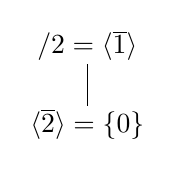
\begin{tikzpicture}[baseline=(current bounding box.center), every node/.style={inner sep=1pt}]
    \node (a) at (0,0.8) {$\ZZ/2\ZZ=\langle \overline{1}\rangle$};
    \node (b) at (0,-0.2) {$\langle\overline{2}\rangle=\{0\}$};
    \draw (a)--(b);
  \end{tikzpicture}
  \end{minipage}
  \begin{minipage}{0.42\linewidth}
  \centering
  \begin{tikzpicture}[baseline=(current bounding box.center), every node/.style={inner sep=1pt}]
    \node (a) at (0,1.2) {$\ZZ/4\ZZ=\langle \overline{1}\rangle$};
    \node (note) at (2.5,1.2) {\small（注意：$\langle\overline{1}\rangle=\langle\overline{3}\rangle$）};
    \node (b) at (0,0.1) {$\langle\overline{2}\rangle$};
    \node (c) at (0,-1.0) {$\langle\overline{4}\rangle=\{0\}$};
    \draw (a)--(b)--(c);
  \end{tikzpicture}
  \end{minipage}
  \end{center}

  \begin{center}
  \begin{tikzpicture}[every node/.style={inner sep=1pt}]
    \node (a) at (0,1.8) {$\ZZ/8\ZZ=\langle\overline{1}\rangle$};
    \node (note) at (3.8,1.8) {\small（注意：$\langle\overline{1}\rangle=\langle\overline{3}\rangle=\langle\overline{5}\rangle=\langle\overline{7}\rangle$）};
    \node (b) at (0,0.7) {$\langle\overline{2}\rangle$};
    \node (c) at (0,-0.4) {$\langle\overline{4}\rangle$};
    \node (d) at (0,-1.5) {$\langle\overline{8}\rangle=\{0\}$};
    \draw (a)--(b)--(c)--(d);
  \end{tikzpicture}
  \end{center}

  一般地，若 $p$ 是素数，则 $\ZZ/p^n\ZZ$ 的格为
  \begin{center}
  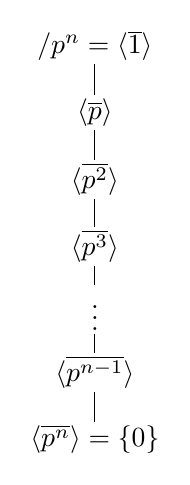
\begin{tikzpicture}[every node/.style={inner sep=1pt}]
    \node (a) at (0,2.8) {$\ZZ/p^n\ZZ=\langle\overline{1}\rangle$};
    \node (b) at (0,1.95) {$\langle\overline{p}\rangle$};
    \node (c) at (0,1.1) {$\langle\overline{p^2}\rangle$};
    \node (d) at (0,0.25) {$\langle\overline{p^3}\rangle$};
    \node (e) at (0,-0.55) {$\vdots$};
    \node (f) at (0,-1.35) {$\langle\overline{p^{n-1}}\rangle$};
    \node (g) at (0,-2.2) {$\langle\overline{p^n}\rangle=\{0\}$};
    \draw (a)--(b)--(c)--(d)--(e)--(f)--(g);
  \end{tikzpicture}
  \end{center}

  \begin{center}
  \begin{minipage}{0.45\linewidth}
  \centering
  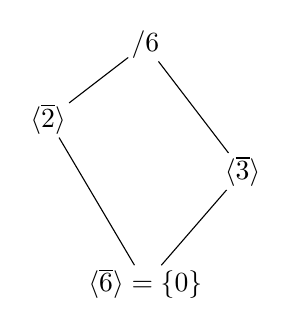
\begin{tikzpicture}[scale=.95, every node/.style={inner sep=1pt}]
    \node (top) at (0,2) {$\ZZ/6\ZZ$};
    \node (a) at (-1.3,1) {$\langle\overline{2}\rangle$};
    \node (b) at (1.3,0.3) {$\langle\overline{3}\rangle$};
    \node (bot) at (0,-1.2) {$\langle\overline{6}\rangle=\{0\}$};
    \draw (top)--(a)--(bot)--(b)--(top);
  \end{tikzpicture}
  \end{minipage}
  \begin{minipage}{0.45\linewidth}
  \centering
  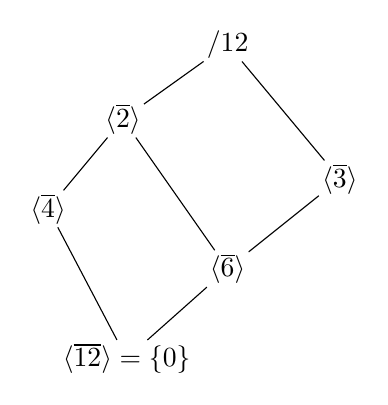
\begin{tikzpicture}[scale=.95, every node/.style={inner sep=1pt}]
    \node (top) at (0,2.2) {$\ZZ/12\ZZ$};
    \node (a) at (-1.4,1.2) {$\langle\overline{2}\rangle$};
    \node (b) at (1.5,.4) {$\langle\overline{3}\rangle$};
    \node (c) at (-2.4,0) {$\langle\overline{4}\rangle$};
    \node (d) at (0,-.8) {$\langle\overline{6}\rangle$};
    \node (bot) at (-1.35,-2.0) {$\langle\overline{12}\rangle=\{0\}$};
    \draw (top)--(a)--(c)--(bot)--(d)--(b)--(top);
    \draw (a)--(d);
  \end{tikzpicture}
  \end{minipage}
  \end{center}

  \item \emph{克莱因四元群}（Viergruppe）$V_4$ 是阶为 $4$ 的群，其乘法表与格为
  \begin{center}
  \begin{tabular}{c@{\qquad}c}
  $\begin{array}{c|cccc}
    \cdot&1&a&b&c\\ \hline
    1&1&a&b&c\\
    a&a&1&c&b\\
    b&b&c&1&a\\
    c&c&b&a&1
  \end{array}$
  &
  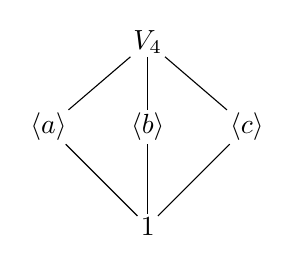
\begin{tikzpicture}[baseline=(current bounding box.center), scale=.9, every node/.style={inner sep=1pt}]
    \node (top) at (0,2) {$V_4$};
    \node (a) at (-1.4,.8) {$\langle a\rangle$};
    \node (b) at (0,.8) {$\langle b\rangle$};
    \node (c) at (1.4,.8) {$\langle c\rangle$};
    \node (bot) at (0,-.6) {$1$};
    \draw (top)--(a)--(bot)--(c)--(top);
    \draw (top)--(b)--(bot);
  \end{tikzpicture}
  \end{tabular}
  \end{center}
  注意 $V_4$ 是阿贝尔群，且不同构于 $Z_4$（为什么？）。我们会看到 $D_8$ 含有一个同构于 $V_4$ 的子群，因此不必检查上述定义的二元运算满足结合律。

  \item $S_3$ 的格为
  \begin{center}
  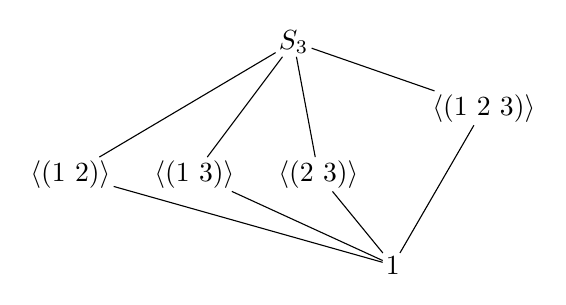
\begin{tikzpicture}[scale=1.05, every node/.style={inner sep=1pt}]
    \node (top) at (0,2.2) {$S_3$};
    \node (a) at (-2.7,.6) {$\langle(1\ 2)\rangle$};
    \node (b) at (-1.2,.6) {$\langle(1\ 3)\rangle$};
    \node (c) at (.3,.6) {$\langle(2\ 3)\rangle$};
    \node (d) at (2.3,1.4) {$\langle(1\ 2\ 3)\rangle$};
    \node (bot) at (1.2,-.5) {$1$};
    \foreach \x in {a,b,c,d} {\draw (top)--(\x); \draw (\x)--(bot);}
  \end{tikzpicture}
  \end{center}

  \item 用通常记号 $D_8=\langle r,s\rangle$，$D_8$ 的格为
  \begin{center}
  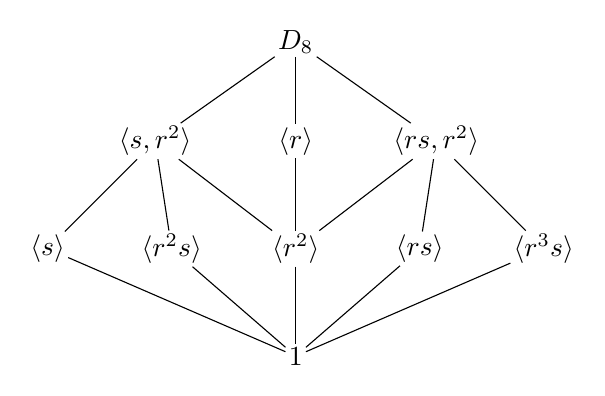
\begin{tikzpicture}[scale=1.05, every node/.style={inner sep=1pt}]
    \node (top) at (0,3) {$D_8$};
    \node (a) at (-1.7,1.8) {$\langle s,r^2\rangle$};
    \node (b) at (0,1.8) {$\langle r\rangle$};
    \node (c) at (1.7,1.8) {$\langle rs,r^2\rangle$};
    \node (d) at (-3,.5) {$\langle s\rangle$};
    \node (e) at (-1.5,.5) {$\langle r^2s\rangle$};
    \node (f) at (0,.5) {$\langle r^2\rangle$};
    \node (g) at (1.5,.5) {$\langle rs\rangle$};
    \node (h) at (3,.5) {$\langle r^3s\rangle$};
    \node (bot) at (0,-.8) {$1$};
    \draw (top)--(a)--(d)--(bot);
    \draw (top)--(b)--(f)--(bot);
    \draw (top)--(c)--(h)--(bot);
    \draw (a)--(e)--(bot);
    \draw (a)--(f);
    \draw (c)--(f);
    \draw (c)--(g)--(bot);
  \end{tikzpicture}
  \end{center}

  \item $Q_8$ 的子群格为
  \begin{center}
  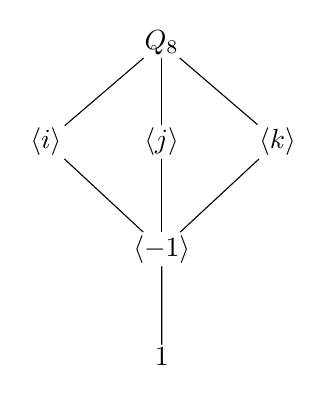
\begin{tikzpicture}[scale=1.05, every node/.style={inner sep=1pt}]
    \node (top) at (0,2.8) {$Q_8$};
    \node (a) at (-1.4,1.6) {$\langle i\rangle$};
    \node (b) at (0,1.6) {$\langle j\rangle$};
    \node (c) at (1.4,1.6) {$\langle k\rangle$};
    \node (d) at (0,.3) {$\langle -1\rangle$};
    \node (bot) at (0,-1) {$1$};
    \draw (top)--(a)--(d)--(bot);
    \draw (top)--(b)--(d);
    \draw (top)--(c)--(d);
  \end{tikzpicture}
  \end{center}

  \item $D_{16}$ 的子群格不是平面图（不能在平面上画出而不使线相交）。它的一种画法是
  \begin{center}
  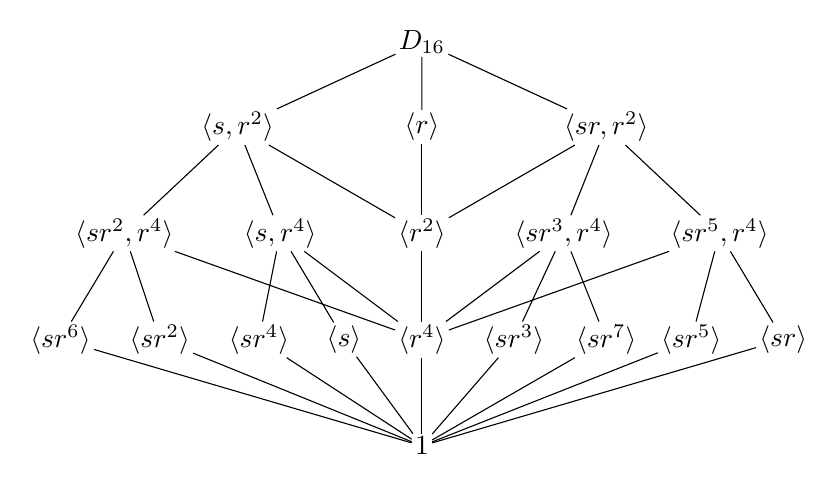
\begin{tikzpicture}[scale=.9, every node/.style={inner sep=1pt}]
    \node (top) at (0,5) {$D_{16}$};
    \node (sr2) at (-2.6,3.8) {$\langle s,r^2\rangle$};
    \node (r) at (0,3.8) {$\langle r\rangle$};
    \node (srr2) at (2.6,3.8) {$\langle sr,r^2\rangle$};
    \node (sr2r4) at (-4.2,2.3) {$\langle sr^2,r^4\rangle$};
    \node (sr4) at (-2,2.3) {$\langle s,r^4\rangle$};
    \node (r2) at (0,2.3) {$\langle r^2\rangle$};
    \node (sr3r4) at (2,2.3) {$\langle sr^3,r^4\rangle$};
    \node (sr5r4) at (4.2,2.3) {$\langle sr^5,r^4\rangle$};
    \node (sr6) at (-5.1,.8) {$\langle sr^6\rangle$};
    \node (sr2s) at (-3.7,.8) {$\langle sr^2\rangle$};
    \node (sr4s) at (-2.3,.8) {$\langle sr^4\rangle$};
    \node (ss) at (-1.1,.8) {$\langle s\rangle$};
    \node (r4) at (0,.8) {$\langle r^4\rangle$};
    \node (sr3) at (1.3,.8) {$\langle sr^3\rangle$};
    \node (sr7) at (2.6,.8) {$\langle sr^7\rangle$};
    \node (sr5) at (3.8,.8) {$\langle sr^5\rangle$};
    \node (sr) at (5.1,.8) {$\langle sr\rangle$};
    \node (bot) at (0,-.7) {$1$};
    \draw (top)--(sr2) (top)--(r) (top)--(srr2);
    \draw (sr2)--(sr2r4) (sr2)--(sr4) (sr2)--(r2);
    \draw (r)--(r2);
    \draw (srr2)--(r2) (srr2)--(sr3r4) (srr2)--(sr5r4);
    \draw (sr2r4)--(sr6) (sr2r4)--(sr2s) (sr2r4)--(r4);
    \draw (sr4)--(sr4s) (sr4)--(ss) (sr4)--(r4);
    \draw (r2)--(r4);
    \draw (sr3r4)--(r4) (sr3r4)--(sr3) (sr3r4)--(sr7);
    \draw (sr5r4)--(r4) (sr5r4)--(sr5) (sr5r4)--(sr);
    \foreach \x in {sr6,sr2s,sr4s,ss,r4,sr3,sr7,sr5,sr} {\draw (\x)--(bot);}
  \end{tikzpicture}
  \end{center}
\end{enumerate}

在理论证明和具体例子中，我们常常只关心给定群的两个（或少数几个）子群及其相互关系。为了把这些关系画出来，我们将画出整个群格的一个\emph{子格}，其中包含相关的上确界与交。这样的子格中的一条不断开的线一般并不表示该线两端之间没有其他子群。这些部分格也会在处理无限群时使用。例如，若只想讨论 $D_{16}$ 的子群 $\langle sr^2,r^4\rangle$ 与 $\langle r^2\rangle$ 的关系，可画出如下子格：
\begin{center}
\begin{tikzpicture}[scale=1.0, every node/.style={inner sep=1pt}]
  \node (top) at (0,4) {$D_{16}$};
  \node (a) at (0,3) {$\langle s,r^2\rangle$};
  \node (b) at (-1.5,1.8) {$\langle sr^2,r^4\rangle$};
  \node (c) at (1.5,1.8) {$\langle r^2\rangle$};
  \node (d) at (0,.6) {$\langle r^4\rangle$};
  \node (bot) at (0,-.5) {$1$};
  \draw (top)--(a)--(b)--(d)--(bot);
  \draw (a)--(c)--(d);
\end{tikzpicture}
\end{center}
注意 $\langle s,r^2\rangle$ 和 $\langle r^4\rangle$ 分别正是这两个子群在 $D_{16}$ 中的上确界与交。

最后，给定一个群的子群格后，计算正规化子和中心化子相对容易。例如，在 $D_8$ 中，可以看出 $C_{D_8}(s)=\langle s,r^2\rangle$，因为先计算得 $r^2\in C_{D_8}(s)$（见第 2 节）。这证明 $\langle s,r^2\rangle\leq C_{D_8}(s)$（注意一个元素总属于它自身的中心化子）。包含 $\langle s,r^2\rangle$ 的子群只有它自身和整个 $D_8$。不可能有 $C_{D_8}(s)=D_8$，因为 $r$ 不与 $s$ 交换（即 $r\notin C_{D_8}(s)$）。于是只剩所声称的一种可能。

\subsection*{练习}

\begin{enumerate}[label=\arabic*.]
  \item 设 $H$ 和 $K$ 是 $G$ 的子群。列出所有可能的只显示 $G$、$1$、$H$、$K$ 及其上确界与交的子格。不同图形的区别是什么？
  \item 在 (a)--(d) 中，列出 $D_{16}$ 中满足给定条件的所有子群：
  \begin{enumerate}[label=(\alph*)]
    \item 包含于 $\langle sr^2,r^4\rangle$ 的子群；
    \item 包含于 $\langle sr^7,r^4\rangle$ 的子群；
    \item 含有 $\langle r^4\rangle$ 的子群；
    \item 含有 $\langle s\rangle$ 的子群。
  \end{enumerate}
  \item 证明 $D_8$ 的子群 $\langle s,r^2\rangle$ 同构于 $V_4$。
  \item 用给定的格找出所有生成 $D_8$ 的元素对（共有 $12$ 对）。
  \item 用给定的格找出所有 $x\in D_{16}$，使得 $D_{16}=\langle x,s\rangle$（共有 $16$ 个这样的元素 $x$）。
  \item 用给定的格帮助求下列群中每个元素的中心化子：
  \[
    \text{(a) }D_8,\qquad
    \text{(b) }Q_8,\qquad
    \text{(c) }S_3,\qquad
    \text{(d) }D_{16}.
  \]
  \item 求 $D_{16}$ 的中心。
  \item 在下列每个群中，求每个子群的正规化子：
  \[
    \text{(a) }S_3,
    \qquad
    \text{(b) }Q_8.
  \]
  \item 画出下列群的子群格：
  \[
    \text{(a) }\ZZ/16\ZZ,
    \qquad
    \text{(b) }\ZZ/24\ZZ,
    \qquad
    \text{(c) }\ZZ/48\ZZ.
  \]
  [参见第 3 节练习 6。]
  \item 通过证明若 $|G|=4$，则 $G\cong Z_4$ 或 $G\cong V_4$，来分类阶为 $4$ 的群。[见第 1.1 节练习 36。]
  \item 考虑具有如下表示的阶为 $16$ 的群：
  \[
    QD_{16}=\langle \sigma,\tau\mid \sigma^8=\tau^2=1,
    \sigma\tau=\tau\sigma^3\rangle
  \]
  （称为阶为 $16$ 的\emph{拟二面体群}或\emph{半二面体群}）。这个群有三个阶为 $8$ 的子群：
  \[
    \langle \tau,\sigma^2\rangle\cong D_8,
    \qquad
    \langle\sigma\rangle\cong Z_8,
    \qquad
    \langle\sigma^2,\sigma\tau\rangle\cong Q_8,
  \]
  并且每个真子群都包含于这三个子群之一。在下列拟二面体群全部子群的格中填入缺失的子群，并用至多两个生成元表示每个子群。（这是另一个非平面格的例子。）

  \begin{center}
  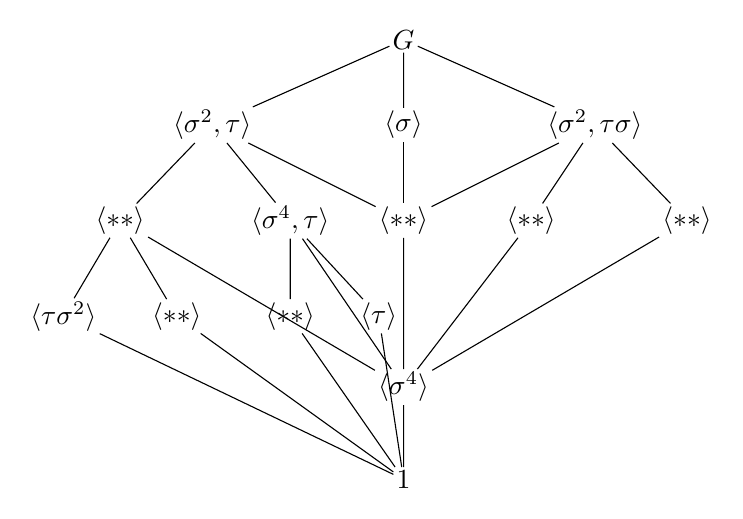
\begin{tikzpicture}[scale=.9, every node/.style={inner sep=1pt}]
    \node (top) at (0,5) {$G$};
    \node (left8) at (-2.7,3.8) {$\langle\sigma^2,\tau\rangle$};
    \node (mid8) at (0,3.8) {$\langle\sigma\rangle$};
    \node (right8) at (2.7,3.8) {$\langle\sigma^2,\tau\sigma\rangle$};
    \node (l1) at (-4.0,2.45) {$\langle **\rangle$};
    \node (l2) at (-1.6,2.45) {$\langle\sigma^4,\tau\rangle$};
    \node (m1) at (0,2.45) {$\langle **\rangle$};
    \node (r1) at (1.8,2.45) {$\langle **\rangle$};
    \node (r2) at (4.0,2.45) {$\langle **\rangle$};
    \node (a) at (-4.8,1.1) {$\langle\tau\sigma^2\rangle$};
    \node (b) at (-3.2,1.1) {$\langle **\rangle$};
    \node (c) at (-1.6,1.1) {$\langle **\rangle$};
    \node (d) at (-.35,1.1) {$\langle\tau\rangle$};
    \node (e) at (0,.1) {$\langle\sigma^4\rangle$};
    \node (bot) at (0,-1.2) {$1$};
    \draw (top)--(left8) (top)--(mid8) (top)--(right8);
    \draw (left8)--(l1) (left8)--(l2) (left8)--(m1);
    \draw (mid8)--(m1);
    \draw (right8)--(m1) (right8)--(r1) (right8)--(r2);
    \draw (l1)--(a) (l1)--(b) (l1)--(e);
    \draw (l2)--(c) (l2)--(d) (l2)--(e);
    \draw (m1)--(e) (r1)--(e) (r2)--(e);
    \draw (a)--(bot) (b)--(bot) (c)--(bot) (d)--(bot) (e)--(bot);
  \end{tikzpicture}
  \end{center}

  下面三个例子导向两个不同构但具有相同子群格的群。

  \item 群
  \[
    A=Z_2\times Z_4=\langle a,b\mid a^2=b^4=1,
    ab=ba\rangle
  \]
  有阶 $8$，并有三个阶为 $4$ 的子群：
  \[
    \langle a,b^2\rangle\cong V_4,
    \qquad
    \langle b\rangle\cong Z_4,
    \qquad
    \langle ab\rangle\cong Z_4,
  \]
  且每个真子群都包含于这三个子群之一。画出 $A$ 的全部子群格，并用至多两个生成元表示每个子群。
  \item 群
  \[
    G=Z_2\times Z_8=\langle x,y\mid x^2=y^8=1,
    xy=yx\rangle
  \]
  有阶 $16$，并有三个阶为 $8$ 的子群：
  \[
    \langle x,y^2\rangle\cong Z_2\times Z_4,
    \qquad
    \langle y\rangle\cong Z_8,
    \qquad
    \langle xy\rangle\cong Z_8,
  \]
  且每个真子群都包含于这三个子群之一。画出 $G$ 的全部子群格，并用至多两个生成元表示每个子群（参见练习 12）。
  \item 设 $M$ 是具有如下表示的阶为 $16$ 的群：
  \[
    \langle u,v\mid u^2=v^8=1,
    vu=uv^5\rangle,
  \]
  （有时称为阶为 $16$ 的\emph{模群}）。它有三个阶为 $8$ 的子群：$\langle u,v^2\rangle$、$\langle v\rangle$ 和 $\langle uv\rangle$，并且每个真子群都包含于这三个子群之一。证明
  \[
    \langle u,v^2\rangle\cong Z_2\times Z_4,
    \qquad
    \langle v\rangle\cong Z_8,
    \qquad
    \langle uv\rangle\cong Z_8.
  \]
  说明 $M$ 的子群格与 $Z_2\times Z_8$ 的子群格相同（参见练习 13），但这两个群不同构。
  \item 描述 $D_{16}$ 中三个阶为 $8$ 的子群各自的同构类型。
  \item 用阶为 $16$ 的拟二面体群的子群格说明，每个阶为 $2$ 的元素都包含在真子群 $\langle\tau,\sigma^2\rangle$ 中（参见练习 11）。
  \item 用阶为 $16$ 的模群 $M$ 的子群格说明集合
  \[
    \{x\in M\mid x^2=1\}
  \]
  是 $M$ 的一个同构于克莱因四元群的子群（参见练习 14）。
  \item 用格帮助求 $QD_{16}$ 中每个元素的中心化子（参见练习 11）。
  \item 用格帮助求 $N_{D_{16}}(\langle s,r^4\rangle)$。
  \item 用 $QD_{16}$ 的子群格（参见练习 11）帮助求正规化子：
  \[
    \text{(a) }N_{QD_{16}}(\langle\tau\sigma\rangle),
    \qquad
    \text{(b) }N_{QD_{16}}(\langle\tau,\sigma^4\rangle).
  \]
\end{enumerate}
